\documentclass{unicam_thesis}
\usepackage[utf8]{inputenc}
\usepackage{listings}
%%%%%%%%%%%%%%%%%%%%%%%%%%%%
% TESI DATI FRONTESPIZIO
%%%%%%%%%%%%%%%%%%%%%%%%%%%%

\title{Analisi e sviluppo di un sistema software\\ per la domotica d'ufficio: il backend di “Proximity System”}

\university{Universit\`a degli Studi di Camerino}%
\school{Scienze e Tecnologie}%
\course{Laurea in Informatica (Classe L-31)}%


\author{Saverio Tosi}%
\advisor{Dott. Francesco De Angelis}%
\coadvisor2{Dott. Francesco Strazzullo}%
\academicyear{2015/2016}%
\matricola{090311}%

%%%%%%%%%%%%%%%%%%%%%%%%%%%%
% FINE DATI FRONTESPIZIO
%%%%%%%%%%%%%%%%%%%%%%%%%%%%

\theoremstyle{definition} \newtheorem{esempio}{Esempio}[chapter]
\theoremstyle{definition}
\newtheorem{definizione}{Definizione}[chapter] \theoremstyle{plain}
\newtheorem{teorema}{Teorema}[chapter]

\graphicspath{{Screenshot/},{Immagini/}}
\bibliography{biblio.bib}
\begin{document}

\maketitle

\tableofcontents
\lstlistoflistings
\listoffigures
\listoftables

\chapter{Introduzione}
\label{chap:intro}

Questa tesi rappresenta la terza ed ultima parte dello stage++\footnote{Lo stage++ è un progetto unico, formato dall'unione di tre esami: project work, stage e tesi.},
realizzato in collaborazione con extrategy, il Prof. Francesco De Angelis e con il collega e amico Marco D'Argenio.
In questo stage ci è stato chiesto di realizzare un'applicazione per la domotica pensata per l'ufficio che prevedesse l'uso dei beacon, ovvero dei piccoli trasmettitori bluetooth che permettono la geolocalizzazione interna negli edifici. 
Proprio per questo motivo, il nome che abbiamo deciso di dare al nostro prodotto è: “Proximity System".

Gli obiettivi che dovevamo raggiungere con questo progetto erano numerosi, ragion per cui, io e Marco, ci siamo divisi il carico in maniera bilanciata e logica.
Io ho trattato tutti gli argomenti inerenti al backend e ai beacon. 
Marco, invece, ha trattato gli argomenti relativi al frontend dell'applicazione e ha studiato il BMC\footnote{Business Model Canvas} del prodotto per vedere la fattibilità dello stesso da un punto di vista economico. 
Questi argomenti non verranno trattati qui, ma nella tesi di Marco:“Analisi e sviluppo di un sistema software per la domotica d'ufficio: il frontend di Proximity System".

In sintesi, il progetto prevede tre parti: 
\begin{enumerate}
\item Il backend in esecuzione su Raspberry PI
\item Una web app per l'amministrazione del sistema
\item Un'app mobile per gestire i dispositivi
\end{enumerate}
Tutte e tre le componenti hanno una cosa in comune, sono tutte scritte in Javascript.

In questa tesi vedremo in dettaglio il primo punto, come utilizzare lo stack MEAN\index{MEAN} per lo sviluppo di applicazioni web rispetto al tradizionale stack LAMP e come le WebSocket possano aumentare drasticamente le performance di un'applicazione real-time.

Il codice completo del progetto è disponibile nei due repository
\begin{enumerate}
\item \url{www.github.com/e-xtrategy/unicam-beacon-server}
\item \url{www.github.com/e-xtrategy/unicam-ionic-beacon-app}
\end{enumerate} 
Il primo contiene sia il backend con le API REST che la web app in Angular.
Il secondo contiene l'App Ionic compatibile con Android, iOS e, parzialmente (almeno per ora), Ubuntu Touch. 

\section{Analisi e progettazione}
La fase di analisi e di progettazione non si è sviluppata in maniera tradizionale, in quanto extrategy basa lo sviluppo di software sulle metodologie agili, più adatte ad ambienti dinamici come lo è il web.
Fra le pratiche promosse da questi metodi ci sono la formazione di team di sviluppo piccoli, cross-funzionali e auto-organizzati, 
lo sviluppo iterativo e incrementale, la pianificazione adattiva, e il coinvolgimento diretto e continuo del cliente nel processo di sviluppo.

Per essere precisi, abbiamo utilizzato un mix tra Scrum e Kanban.
Con Scrum\cite{scrum}\index{Scrum}, il prodotto viene realizzato tramite una serie di iterazioni a intervalli regolari chiamate sprint\index{Sprint} che danno al team un framework per consegnare al cliente del codice con una cadenza costante.
L'idea è quella che degli sprint frequenti rinforzano l'importanza di fare delle giuste stime e permettono di ricevere feedback in tempo reale sul lavoro svolto.
Ogni sprint è caratterizzato da questi quattro riti:
\begin{enumerate}
\item \textbf{Pianificazione}: un incontro iniziale in cui definire cosa fare con lo sprint corrente.
\item \textbf{Scrum giornaliero}: un mini incontro giornaliero della durata di una decina di minuti per sincronizzare il team. 
\item \textbf{Demo}: un incontro per illustrare il lavoro svolto dal team.
\item \textbf{Retrospettiva}: una revisione di ciò che si è stato fatto per farlo meglio la volta successiva.
\end{enumerate} 

Kanban\cite{kanban}\index{kanban} ci è d'aiuto durante gli sprint per tenere sott'occhio tramite una board l'avanzamento del nostro progetto.
Con questa metodologia il lavoro dell'intero team gira intorno alla kanban board, uno strumento utilizzato per visualizzare e ottimizzare il flusso del lavoro per tutto il team.
Mentre delle lavagne o intere pareti sono popolari per molti team, le board virtuali sono una caratteristica cruciale per lo sviluppo di software con le metodologie agile per la loro tranciabilità, facilità di collaborazione e accessibilità da diverse località.

Al di là che la board sia fisica o digitale, la sua funzione è quella di assicurare che il lavoro del team sia visualizzato, che il flusso sia standardizzato e che ogni imprevisto sia immediatamente visualizzato e risolto.
una kanban board di base ha tre step: To Do, In Progress e Done.
È ovvio che non c'è nessun vincolo sulla gestione del flusso e esso dipende da diversi fattori.
La metodologia kanban è basata sulla trasparenza del lavoro svolto e sulla comunicazione,
perciò  la kanban board dovrebbe essere vista come unica fonte di verità per il team. 

Questa impostazione crea l'esigenza di una piattaforma in grado di tenere traccia dello sviluppo del software e delle user-stories da implementare, capace anche di coordinare gli sviluppatori dedicati a quel caso.
Nonostante kanbanize probabilmente è una delle soluzione online più adatte ad implementare la metodologia Kanban, abbiamo scelto Trello perché il nostro piccolo team non necessita di applicare alla lettera Kanban con tutte le procedure consigliate per la gestione del flusso, e una semplice todo list era più che sufficiente.
 
Trello\index{Trello}\cite{trello} é un gestore di progetti basato sul web, originariamente realizzato da Fog Creek Soft-ware nel 2011.
In questo caso il progetto è rappresentato da schede, che contengono liste corrispondenti ad elenchi di attività. 
Le liste sono formate da card, che rappresentano le singole attività. 
Le card sono tenute a passare da una lista all'altra, tramite la funzione drag-and-drop; per via del generico flusso di una card, essa dovrebbe passare dalla lista delle cose da fare a quelle fatte, al momento del passaggio dall'idea alla realizzazione dell'attività in questione.
Nello specifico le card rappresentano le user-stories, funzionalità utile al raggiungimento di un obiettivo di business, una descrizione appositamente non dettagliata che il software deve avere e che alimenti la discussione tra il cliente/utente e lo sviluppatore.
Più programmatori possono essere assegnati alle card, ed insieme alle relative schede, possono essere raggruppati in organizzazioni differenti. 
Ogni card può accettare commenti, allegati, voti, date di scadenza e liste di controllo.
La suddivisione di un progetto in schede/liste, a loro volta suddivise in card formano una gerarchia di dati su misura che facilita la gestione efficace dei progetti stessi, nonché delle attività dell'intera organizzazione.
\begin{figure}[h]
\centering
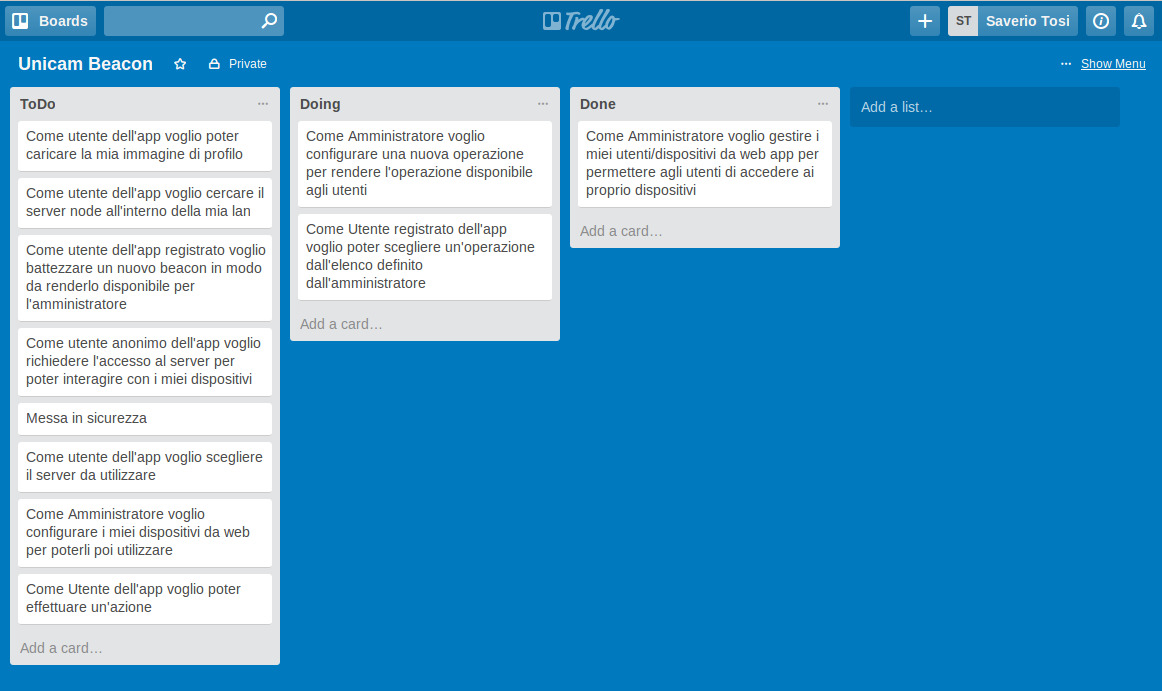
\includegraphics[scale=0.35]{Immagini/trello.png} 
\caption{Il nostro Trello, nella fase iniziale del progetto}
\end{figure}

\subsection{Analisi dei requisiti}
Si vuole realizzare un sistema per la domotica per d'ufficio, che oltre ad essere comandato con un'app, utilizzi i beacon per eseguire dei comandi automatizzati.

Il backend deve essere caricato su un RaspberryPI 2 e deve fornire i servizi REST\index{REST} sia per la webapp che per l'app mobile. 
Inoltre, dove essere in grado di comunicare con il mondo esterno: sia con input che con degli output.
Per il prototipo, gli input saranno simulati con l'utilizzo di bottoni, nel prodotto finito essi saranno sostituiti con degli interruttori e dei sensori.
Gli output devono pilotare dei relè monostabili che permetteranno di comandare l'accensione/spegnimenti di luci, l'apertura di porte e di cancelli.

Il pannello di amministrazione è rappresentato dalla webapp a cui potrà accedere soltanto l'admin. 
Essa permette di gestire gli utenti dell'app dandogli e togliendogli privilegi, creare nuovi dispositivi da associare ai vari GPIO del RaspberryPI e di configurare il modo in cui gli utenti possono interagire con i dispositivi: in maniera manuale, automatica(tramite beacon) o se per poter controllare il dispositivo è necessario trovarsi nelle vicinanze di esso. 

L'ultima componente è l'app mobile. 
Chi scaricherà l'app dovrà per prima cosa impostare l'indirizzo del server, se non si conosce l'indirizzo deve essere possibile fare una scansione della rete locale per trovare i backend attivi nella propria LAN. 
Una volta che si è connessi al server si può proseguire con il login/registrazione. 
La registrazione non abilita l'utente all'utilizzo di Proximity System, l'utente non potrà far nulla finché l'admin non gli dà i permessi per utilizzare l'app. 
Con l'app un utente ha due funzionalità: la prima è poter cercare nuovi beacon da segnalare all'amministratore; la seconda è interagire con i propri dispositivi.

\subsubsection{FURPs+}
Per descrivere i requisiti in maniera più formale utilizzeremo il modello FURPS+\index{FURPS+}\cite{furps} creato da Hewlett-Packard.
FURPS è un acronimo per dividere i requisiti in categorie e sottocategorie:
\begin{itemize}
\item \textbf{F}unctionality(FUN): Capability, Security, Reusability;
\item \textbf{U}sability(USA): Human Factors, Aesthetics, Consistency, Documentation, Responsiveness;
\item \textbf{R}eliability(REL): Availability, Failure Extent and Time-Length, Predictability, Accuracy;
\item \textbf{P}erformance(PER): Speed, Efficiency, Resource Consumption, Throughput, Capacity, Scalability;
\item \textbf{S}upportability(SUP): Testability, Flexibility, Installability, Localizability;
\end{itemize}
Il "+" è stato aggiunto successivamente per estendere l'acronimo ad altri attributi.

I requisiti funzionali descrivono azioni specifiche che il sistema deve essere in grado di effettuare, senza alcun vincolo.
Quindi, specificano il comportamento del sistema.
Una lista di questi verrà fatta di seguito con un ID e una breve descrizione.
Ogni ID avrà il seguente formato "\textbf{FUN-nn}" dove \textbf{nn} è un numero che identifica il requisito.
\begin{longtable}{|c|l|}
% intestazione iniziale
\hline
\multicolumn{1}{|c|}{\textbf{ID}} & \multicolumn{1}{c|}{\textbf{Descrizione}} \\
\endfirsthead
% intestazione normale
\multicolumn{2}{l}{\footnotesize\itshape\tablename~\thetable:
continua dalla pagina precedente} \\
\hline
\multicolumn{1}{|c|}{\textbf{ID}} & \multicolumn{1}{c|}{\textbf{Descrizione}} \\
\endhead
% piede normale
\multicolumn{2}{r}{\footnotesize\itshape\tablename~\thetable:
continua nella prossima pagina} \\
\endfoot
% piede finale
\multicolumn{2}{r}{} \\
\endlastfoot
\hline
FUN-01 & L'app deve permettere di utilizzare i proprio dispositivi.\\
\hline
FUN-02 & L'app deve permettere ai nuovi utenti di registrarsi e ai vecchi di\\
& effettuare il login.\\
\hline
FUN-03 & L'app deve permettere agli utenti di segnalare nuovi beacon\\
& all'amministratore.\\
\hline
FUN-04 & L'app deve permettere agli utenti di ricercare Proximity System\\
& all'interno della propria LAN.\\
\hline
FUN-05 & L'app deve permettere di settare l'indirizzo del server.\\
\hline
FUN-06 & L'app deve eseguire automaticamente le operazioni con i beacon\\
& associati.\\
\hline
FUN-07 & La webapp deve permettere il login solo all'amministratore.\\
\hline
FUN-08 & La webapp deve permettere la gestione manuale dei GPIO.\\
\hline
FUN-09 & La webapp deve permettere la gestione degli utenti: modifica,\\
& blocco/sblocco.\\
\hline
FUN-10 & La webapp deve permettere la gestione dei dispositivi: creazione,\\
& eliminazione.\\
\hline
FUN-11 & La webapp deve permettere di configurare le azioni, cioè di associare\\
& ai dispositivi: permessi, beacon, modalità di attivazione e input.\\
\hline
FUN-12 & Il backend deve fornire i servizi REST per la webapp, per l'app\\
& e qualsiasi software che potrà essere sviluppato in un secondo\\
& momento.\\
\hline
FUN-13 & Il backend deve poter pilotare dei relè che a loro volta\\
& comanderanno i vari dispositivi.\\
\hline
FUN-14 & Il backend deve deve essere in grado di leggere gli input esterni,\\
& che per il prototipo saranno simulati da dei bottoni.\\
\hline
\caption{Requisiti funzionali.}
\label{tab:req:fun} \\
\end{longtable} 

Passiamo ora ai requisiti non-funzionali, ovvero quelli che descrivono gli attributi del nostro sistema. 
Ogni requisito è identificato dall'ID "\textbf{XXX-nn}" dove \textbf{XXX} identifica il tipo mentre \textbf{nn} è un numero sequenziale che identifica il requisito.
\begin{longtable}{|c|l|}
% intestazione iniziale
\hline
\multicolumn{1}{|c|}{\textbf{ID}} & \multicolumn{1}{c|}{\textbf{Descrizione}} \\
\endfirsthead
% intestazione normale
\multicolumn{2}{l}{\footnotesize\itshape\tablename~\thetable:
continua dalla pagina precedente} \\
\hline
\multicolumn{1}{|c|}{\textbf{ID}} & \multicolumn{1}{c|}{\textbf{Descrizione}} \\
\endhead
% piede normale
\multicolumn{2}{r}{\footnotesize\itshape\tablename~\thetable:
continua nella prossima pagina} \\
\endfoot
% piede finale
\multicolumn{2}{r}{} \\
\endlastfoot
\hline
USA-01 & L'app deve essere semplice da usare.\\
\hline
USA-02 & Sia l'app che la webapp devono rispettare criteri di accessibilità\\
\hline
PER-01 & Sia l'app che la webapp devono poter essere utilizzate soltanto\\
& all'interno della propria LAN\\
\hline
SUP-01 & Il backend deve supportare l'interazione con software di terze-\\
& parti.\\
\hline
\caption{Requisiti non funzionali.}
\label{tab:req:non} \\
\end{longtable} 

\subsubsection{Use Case}
\begin{figure}[h]
\centering
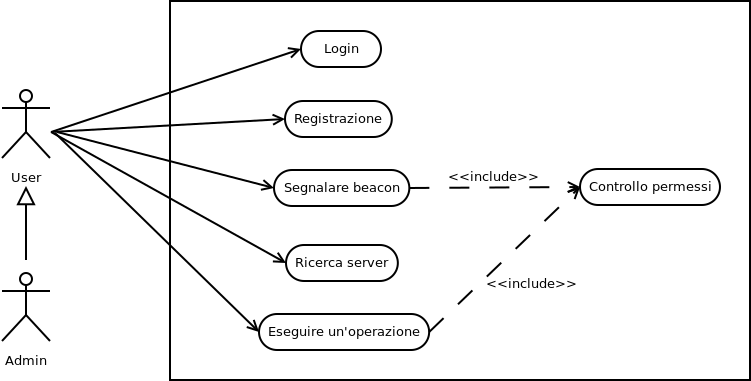
\includegraphics[width=1\textwidth]{Immagini/usecaseApp.png} 
\caption{Use case dell'app}
\end{figure}

Dallo use case dell'app possiamo notare come le funzionalità messe a disposizione dell'utente siano le stesse sia se esso è un utente normale che un admin.
Cambia soltanto il numero delle operazioni messe a disposizione dell'utente che varia a seconda dei permessi.

\begin{figure}[h]
\centering
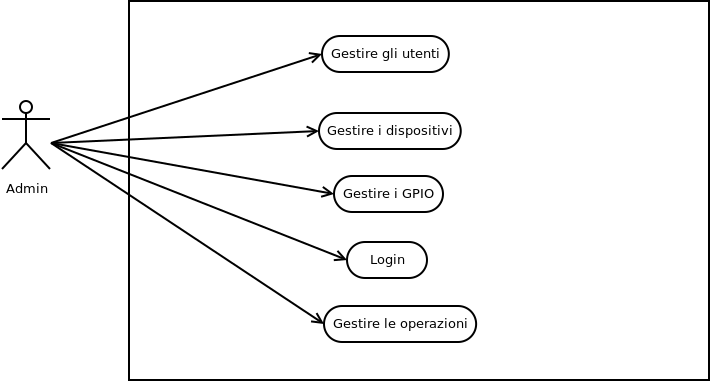
\includegraphics[width=1\textwidth]{Immagini/usecaseWebApp.png} 
\caption{Use case della webapp}
\end{figure}

Alla webapp, invece, può accedere solamente chi ha i massimi privilegi e da essa si può gestire l'intero sistema.
\section{Miglioramento dell'esperienza utente}
Dopo una prima stesura del codice e la realizzazione di un primo prototipo,
abbiamo deciso migliorare l'esperienza utente dando la possibilità al server di inviare notifiche push ai client.
Per fare ciò, abbiamo utilizzato le WebSocket, una delle funzionalità più interessanti introdotta con l'HTML5.

Nel Capitolo \ref{chap:websocket} illustreremo come sia possibile migliorare le  prestazione di una generica WebApp che fornisce dei dati in tempo reale, per poi dimostrare come sia semplice utilizzare tale specifica, sopratutto se si utilizzano delle libreria ad hoc come Socket.io. 
\chapter{IoT}
In questo capitolo andremo a vedere per prima cosa cos'è l'internet delle cose, per poi descrivere la board che abbiamo utilizzato per realizzare il nostro progetto. 

\section{Il futuro delle smart home}
Tutti noi abbiamo sentito parlare, almeno una volta, dell'internet delle cose,
ma in pochi sanno dare una definizione precisa di che cosa sia l'IoT.
Questo perché una definizione rigorosa ad oggi non esiste.
Quello che si intende per Internet of Things è l'estensione della rete ad un numero sempre crescente di dispositivi, o meglio oggetti.
L'insieme di questi: termostati, robot, droni, smart tv, lavastoviglie e molti altri elettrodomestici; rappresenta una solida base per la costruzione di vere e proprie case intelligenti.

L'IoT sta prendendo, giorno dopo giorno, una fetta di mercato sempre più ampia, evolvendosi in fretta e senza seguire standard e protocolli ben specifici. 
Marteen Ector\footnote{Marteen Ectors è uno dei massimi esponenti dell'IoT di  Canonical} ha scritto un articolo\cite{smart} in cui evidenzia dei possibili problemi relativi al futuro di questi oggetti intelligenti.
In particolare si chiede se ci troviamo in una di queste ere:
\begin{itemize}
\item Internet of Useless Things era
\item Internet of Isolated Things era
\item Internet of Insecure Things era
\item Internet of Smart Cheap Things era
\item Internet of App-Enabled Things era
\end{itemize}
Andiamo ad analizzare ogni singola era singolarmente. 
Molti di questi oggetti sono \emph{inutili}, o quasi. Si pensi ad una semplice lampadina, è bello poterla pilotare senza doversi muovere dal divano, ma il problema che risolve è banale.

Non tutti questi smart device parlano la stessa lingua. Prodotti di costruttori diversi usano protocolli diversi \emph{isolandosi} l'un l'altro.

Ci capita spesso di vedere falle di sicurezza che permettano a dei semplici "smanettoni" di accedere senza troppi problemi al microfono e alla webcam della nostra smart tv, anche delle marche più famose.
Siamo sicuri che vogliamo una casa \emph{insicura}?

Il quarto punto rappresenta in realtà un vantaggio dato dal costo delle componenti elettroniche che si sta abbassando drasticamente.
Grazie a ciò è possibile acquistare dei mini-pc per pochi euro. 
Una generica casa, con l'ausilio di questi dispositivi e di qualche sensore, può raccogliere più informazioni di quante ne raccoglieva google 10 anni fa.

Infine, per ogni oggetto che compriamo, troviamo la relativa app sullo store che permette di utilizzare il dispositivo che altrimenti sarebbe inutilizzabile.

Prendendo atto di queste considerazioni e del fatto che il nostro sistema deve adattarsi più all'uso in ufficio che in una casa, abbiamo deciso che il nostro sistema deve avere le seguenti caratteristiche:
\begin{enumerate}
\item \textbf{Open source}: per dare la possibilità a chiunque di migliorarlo e di integrarlo con i propri dispositivi;
\item \textbf{Centralizzato}: non vogliamo avere tanti oggetti intelligenti,
ma uno centrale che ne controlli tanti "stupidi". Questa soluzione non è adatta per spazi ampi come una casa in cui comporterebbe un alto costo per il cablaggio, ma è adatta a singole stanze come un ufficio. 
\end{enumerate} 

\section{Raspberry}
Raspberry è un piccolo calcolatore elettronico dalle dimensioni di una
carta di credito sviluppato nel Regno Unito dalla Raspberry Pi
Foundation. Lo scopo di questa fondazione è quello di sviluppare un
dispositivo economico, che ha la capacità di stimolare l'insegnamento
dell'informatica e della programmazione nelle scuole. La scheda è stata
progettata per ospitare sistemi operativi basati su un kernel linux, tra i
più usati troviamo:
\begin{itemize}
\item Raspbian
\item Ubuntu mate
\item Snappy Ubuntu Core
\item Windows 10 IoT Core
\end{itemize}
Per quanto riguarda i componenti hardware, esso ha la stessa struttura
dei moderni Personal Computer. Raspberry Pi rispetta perfettamente il
modello di Von Neumann, nella quale si individuano quattro componenti
fondamentali: l'unita di elaborazione e controllo, la memoria, il sistema
di ingresso/uscita, il sistema di interconnessione. Inizialmente esistevano tre modelli di Raspberry Pi:
\begin{enumerate}
\item Model A, consigliato per i progetti embedded;
\item Model B, consigliato per l'utilizzo nelle scuole;
\item Model B+, potenziamento del Model B.
\end{enumerate}
Successivamente sono uscite nuove versioni del model B, caratterizzate da più RAM e una CPU migliore, che prendono il nome di Rasperry PI 2 e 3.
Per il nostro progetto abbiamo scelto di utilizzare il Raspberry PI 2 in
quanto è il dispositivo che apre a maggiori possibilità. Il Raspberry Pi 2,
infatti, è dotato di 4 porte USB, un connettore femmina RJ45
10/100BaseT, lettore MicroSD, connettore display DSI, presa HDMI,
connettore fotocamera CSI, un jack da 3,5mm e il cip Broadcom
BCM2836 con processore quad-core Cortex-A7 affiancato da 1024 MB di
memoria RAM.
\begin{figure}[h]
\centering
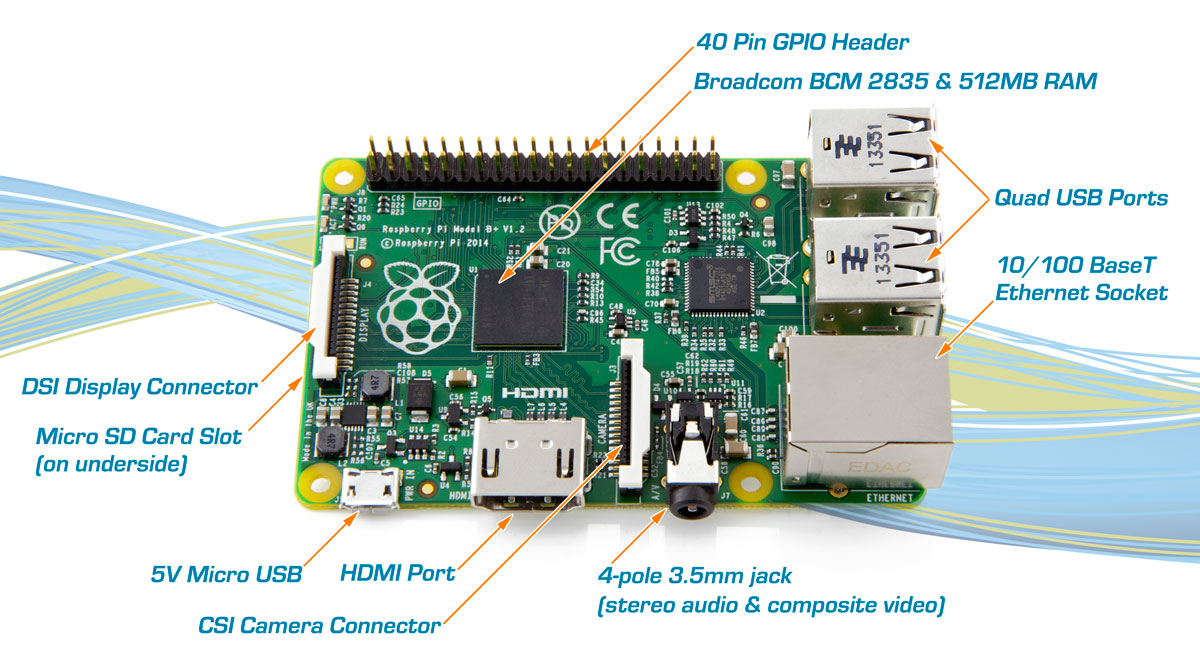
\includegraphics[scale=0.3]{Immagini/raspberry.png}
\caption{Raspberry PI 1 Model B+}
\end{figure}

\subsection{Perchè Raspberry}

Come già descritto nel capitolo \ref{chap:intro}, il prodotto che dobbiamo realizzare non solo deve essere in grado di far girare un webserver, ma deve anche essere in grado di comunicare con il mondo esterno. Raspberry Pi si è rilevato perfetto per questo scopo.
Essendo un dispositivo low cost che però ha sia un processore discreto che la possibilità di comunicare con relè e sensori, in quanto è dotato di ben 40 GPIO.
\chapter{Beacon}
\label{chap:beacon}
Un beacon è una piccola antenna trasmettitore
bluetooth, che lavora alla frequenza standard di 2,4 ghz (la stessa del Wi-fi, per intendersi). Un beacon può inviare soltanto una piccola stringa di
codice, grande qualche manciata di byte, che funge da identificatore del
beacon stesso.

Nel corso degli anni le tipologie di beacon sono aumentate col trascorrere del tempo. Ad oggi, le tre principali tipologie di beacon sono:
\begin{enumerate}
\item iBeacon\index{iBeacon} - Apple
\item EddyStone - Google
\item AltBeacon - Open
\end{enumerate}

Il prodotto della Apple è stato il primo ad entrare nel mercato e per questo è il più diffuso in commercio.
Degli iBeacon verrà fatta una panoramica più ampia nel prossimo paragrafo, per il momento diciamo soltanto che prevede un solo tipo di frame.
EddyStone è un prodotto Google che funziona sia con Android che con iOS. La principale differenza rispetto al prodotto Apple, è la possibilità di scegliere tra due diversi tipi frame da inviare in broadcast. Per finire, AltBeacon nasce con l'esigenza di creare un protocollo per i beacon che sia aperto e che faccia dell'interoperabilità il suo punto di forza.
\section{iBeacon}
iBeacon technology\cite{apple}, introdotta con iOS7, è una tecnologia che permette di migliorare la localizzazione per app.
Utilizzando il Bluetooth Low Energy (BLE), un device che supporta gli iBeacon può essere utilizzato per stabilire se esso è dentro la regione di un determinato oggetto. 
Quindi, Permette ad un dispositivo iOS di determinare quando quest'ultimo entra o esce da una regione, con una stima della prossimità dal beacon.

Se si è interessati ad utilizzare gli ibeacon, si rientra in almeno una delle seguenti categorie di persone:
\begin{enumerate}
\item \textbf{App Developers}
\\Se si vuole migliorare la geo-localizzazione di un'app, si può utilizzare il Core Location APIs in iOS per ricevere notifiche quando un dispositivo entra ed esce dalla regione di un beacon e per stimare la prossimità dal beacon stesso. 
Tutto quello di cui si ha bisogno è incluso in iOS SDK.
\item \textbf{Si vuole utilizzare un dispositivo con la tecnologia iBeacon}
\\Se sei interessato ad utilizzare il logo di iBeacon, ma non sei un produttore di iBeacon, dovrai ottenere una licensa del logo prima di utilizzarlo.
\url{https://developer.apple.com/ibeacon/}   
\item \textbf{Persone che vogliono creare dispositivi con la tecnologia iBeacon}
\\Se sei interessato a costruire dispositivi con iBeacon technology, avrai bisogno di ottenere una licenza da Apple prima di realizzarli. 
Con la licenza hai l'accesso a specifiche tecniche  ed il permesso ad utilizzare il logo iBeacon. 
\end{enumerate}
Un iBeacon advertisement invia le seguenti informazioni via BLE:
\begin{table}[htbp]
\begin{center}
\begin{tabular}{|l|l|l|}
\hline
Campo & Dimensione & Descrizione \\
\hline
UUID & 16 bytes & Lo sviluppatore dovrebbe definirne uno\\
& & per la propria app e utilizzo \\
\hline
Major & 2 bytes & Indica uno specifico caso d'uso dell'iBeacon\\
\hline
Minor & 2 bytes & Suddivide ulteriormente la regione\\
\hline
\end{tabular}
\end{center}
\caption{iBeacon advertisement}
\label{tab:table}
\end{table}
\\UUID, major e minor identificano unicamente il beacon. 
Un UUID può essere generato utilizzando il comando \texttt{uuidgen} da terminale in OS X, o tramite  la classe NSUUID.
La seguente tabella mostra come questi valori possano essere utilizzati da una catena di negozi. 
\begin{table}[htbp]
\begin{center}
\begin{tabular}{|c|c|c|c|}
\hline
Negozio & Ancona & Jesi & Camerino \\
\hline
UUID &
\multicolumn{3}{c|}{D9B9EC1F-3925-43D0-80A9-1E39D4CEA95C} \\
\hline
Major & 1 & 2 & 3\\
\hline
Minor - Vestiti  & 10 & 10 & 10\\
\hline
Minor - Scarpe & 20 & 20 & 20\\
\hline
Minor - Intimo & 30 & 30 & 30\\
\hline
\end{tabular}
\end{center}
\caption{Esempio utilizzo UUID, major e minor}
\label{tab:table}
\end{table}
Utilizzando queste informazioni, un dispositivo iOS può identificare quando entra ed esce da un negozio e in che tipologia di negozio si trova. 
\\
iBeacon utilizzano il BLE, perciò richiede un iPhone 4s(o superiori), iPod touch(quinta generazione), iPad(terza generazione o iPad mini).
\subsection{Privacy and Location}
Dato che la tecnologia iBeacon è parte del Core Location, le stesse autorizzazioni sono richieste per poter essere utilizzata(vedi Figura \ref{fig:autorizzazioni}).
L'utente visualizzerà lo stesso alert quando un'applicazione tenterà di utilizzare le API di iBeacon\footnote{NOTA: Ciascun pacchetto Bluetooth che è associato con gli iBeacon sarà escluso dalle API del CoreBluetooth, nonostante ciò, senza attivare il Bluetooth le API di iBeacon non funzioneranno.}.
\begin{figure}[t]
\centering
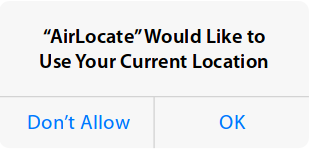
\includegraphics[scale=0.6]{Immagini/alert.png}
\caption{Autorizzazioni iOS} 
\label{fig:autorizzazioni}
\end{figure}\\
Come quando è attivo il GPS, quando utilizziamo la tecnologia iBeacon sarà presente una freccia nella status bar.
\subsection{Precisione degli iBeacon}
Per migliorare la user experience, è importante prendere in considerazione come il segnale dei beacon viene letto e utilizzato per determinare la distanza da esso. 
Quando un dispositivo iOS rileva un beacon, utilizza la potenza del segnale (RSSI - Received Signal Strength Indication)\index{RSSI} per determinare la proximity dal beacon.
Più potente è il segnale e migliore sarà la stima fatta dal device.
La potenza del segnale è generalmente correlata dalla distanza fra il beacon e il dispositivo. In una condizione ideale la vicinanza del dispositivo dal beacon migliora la precisione.
Quando un dispositivo è lontano dal beacon, la potenza del segnale sarà minore rispetto a quando è vicino. 
Minore è la potenza del segnale, minore sarà la precisione nel calcolo della prossimità. 
Lo stesso accade con il GPS.
Come il dispositivo si avvicina al beacon, il segnale diventa più forte e di conseguenza migliora la precisione della distanza.
Come per il segnale GPS, un oggetto fisico può bloccare il segnale del beacon. L'attenuazione del segnale, o semplicemente la perdita di intensità, può essere causata da molti fattori. 
Anche il corpo umano può attenuare il segnale Bluetooth. Basta, per esempio, dare le spalle al beacon per diminuire la precisione del dispositivo nel calcolare la distanza dal beacon.\\
Quando si costruisce un'applicazione che utilizza GPS o beacon, è importante prendere in considerazione la precisione.
Il valore riportato dall'oggetto Core Location, indica il livello di incertezza, o margine di errore misurato in metri. 

\subsection{Monitoraggio regioni}
In maniera simile al monitoraggio di regioni con geofence, un'applicazione può richiedere di ricevere una notifica quando un dispositivo entra o lascia una regione definita da un beacon. 
Quando si crea la richiesta si deve specificare l'UUID dell'iBeacon advertisement. Mentre un'applicazione può monitorare un numero limitato di 20 regioni, usando un singolo UUID in più zone, un dispositivo può monitorare svariate zone contemporaneamente.

In aggiunta all'UUID, un applicazione può selezionare il major ed il minor per rendere più specifica la regione da monitorare.

Come per il monitoraggio di regioni con il GPS, quando un utente entra o esce da una regione l'applicazione riceverà una notifica. 
Se l'applicazione non è in esecuzione(per esempio se è stata terminate per necessità di ram da parte del sistema), l'applicazione verrà lanciata in backgroud e gli verrà inoltrata la notifica. 
Un'importante considerazione sta nel fatto che se l'utente disabilita "Background App Refresh" allora l'app non verrà riavviata e quindi non riceverà le notifiche.

\subsection{Ranging}
iOS 7 ha introdotto un nuovo set di API per determinare approssimativamente la prossimità utilizzando iBeacon technology, processo conosciuto come "Ranging". 
Basandosi sui più comuni scenari, iOS applica dei filtri alla precisione calcolata per determinare una stima della prossimità dal beacon.
Questa stima è indicata utilizzando uno dei seguenti stati di prossimità:
\begin{table}[htbp]
\begin{center}
\begin{tabular}{|l|p{9cm}|}
\hline
Proximity State & Descrizione \\
\hline
Immediate & Indica l'immediata vicinanza del dispositivo al beacon \\
\hline
Near & Se non ci sono ostacoli tra il beacon ed il dispositivo, indica una distanza approssimativa che va da 1 a 3 metri. \\
\hline
Far & Questo stato indica che un beacon è stato rilevato ma non si è in grado di determinare se si è Near o Immediate. 
Un'importante considerazione è che questo stato non implica che si è lontani dal beacon.\\
\hline
Unknow & La prossimità dal beacon non può essere determinato.
Questo può indicare che il ranging è appena iniziato. \\
\hline
\end{tabular}
\end{center}
\caption{Proximity state}
\label{tab:table}
\end{table}

\subsection{Physical limitations}
I dispositivi iBeacon utilizzano il Bluetooth Low Energy\index{BLE} per inviare i messaggi.
BLE lavora ad una frequenza di 2.4GHz e può essere soggetto ad attenuazioni da qualsiasi oggetto fisico come pareti, porte o qualsiasi altro oggetto. La frequenza 2,4 GHz può essere ostacolata anche dall'acqua, ciò significa che anche le persone attenuano il segnale. Come detto precedentemente, quando il segnale ricevuto è debole, diminuisce la capacità del dispositivo di calcolare una stima della prossimità.
\subsection{Calibrazione}
Per migliorare la user experience, un aspetto fondamentale è la calibrazione dei beacon nel vostro sistema.
È consigliato eseguirla per ogni singolo dispositivo.
Il calcolo della distanza da parte del Core Location è effettuato utilizzando il valore Measured Power ottenuto, appunto, con la calibrazione. 
Per eseguirla dobbiamo:
\begin{enumerate}
\item Installare il beacon;
\item Utilizzando un dispositivo con iOS 7 o superiore con il Bluetooth 4.0, campionare la potenza del segnale ad un metro di distanza per un minimo di 10 secondi. In questa fase bisogna ricordarsi di tenere il dispositivo  in verticale e di lasciare libera la metà superiore del device.
\item Muovere il dispositivo avanti e indietro lentamente per 30cm mantenendo l'orientamento e la distanza dal beacon(vedi Figura \ref{fig:calibrazione}). 
\begin{figure}[htbp]
\centering
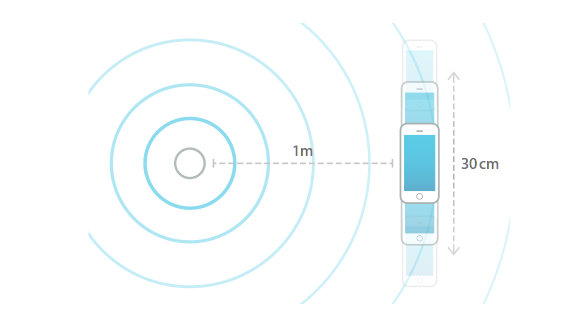
\includegraphics[scale=0.6]{Immagini/fig5.png}
\caption{Calibrazione} 
\label{fig:calibrazione}
\end{figure}\\
\item Calcolare la media dei valori \textit{rssi} registrati per ottenere la \textbf{Measured Power};
\item Applicare il valore di \textbf{Measured Power} al beacon;
\end{enumerate}
Dato che il sistema circostante può influire sulla frequenza del bluetooth, è importante ripetere la procedura per ogni beacon installato. 
\subsection{UUID}
Un \textbf{universally unique identifier}(UUID)\index{UUID} definito in RFC 4122\cite{RFC4122} è un identificatore standard usato per la costruzione di applicazioni.
Esso è semplicemente un numero rappresentato da 128 bit.
Il significato di ogni bit è definito nella specifica di ciascuna delle sue varianti.

Per essere letti anche dagli esseri umani, molti sistemi lo rappresentano in esadecimale inserendo dei caratteri dash al suo interno. Un esempio:
\textbf{de305d54-75b4-431b-adb2-eb6b9e546014} 

L'obiettivo degli UUID è quello di distribuire sistemi con un id univoco senza un'unità centrale di controllo. In questo contesto la parola univoco prende il significato di "praticamente univoco" e non garantisce niente. 
Chiunque può creare un UUID ed utilizzarlo per identificare qualcosa sapendo che le probabilità che qualcun altro generi lo stesso UUID sono veramente basse, se non nulle.

Un UUID è formattato secondo le specifiche delle varianti.
Esistono 5 varianti di UUID:
\begin{enumerate}
\item Version 1 (MAC address \& data-time)
\item Version 2 (DCE Security);
\item Version 3 (MD5 hash \& namespace);
\item Version 4 (random);
\item Version 5 (SHA-1 hash \& namespace).
\end{enumerate}

Se ai 128 bit togliamo i due bit che identificano RFC 4122 e i 4 che identificano la versione, abbiamo che gli UUID generati hanno 122 bit random.
La possibilità che due UUID abbiamo lo stesso identico valore può essere calcolata utilizzando il calcolo della  probabilità(il problema del compleanno).
\begin{equation}
p(n)\cong1-e^{-\frac{n^2}{2-2^x}}
\end{equation}
Questa è la probabilità di una collisione calcolando $n$ UUID, con $x = 122$:
\begin{table}[htbp]
\begin{center}
\begin{tabular}{|c|c|}
\hline
n & probabilità\\
\hline
$65.719.476.736 = 2^{36}$ & $0,0000000000000004 = 4( 10^{-16})$\\
\hline
$2.199.023.255.552 = 2^{41}$ & $0,0000000000005 = 5( 10^{-13})$\\
\hline
$70.368.744.177.664 = 2^{46}$ & $0,0000000005 = 5( 10^{-10})$\\
\hline
\end{tabular}
\end{center}
\caption{Probababilità collisione UUID}
\label{tab:table}
\end{table}
\subsection{ngCordova}
ngCordova\index{ngCordova} mette a disposizione un plugin che permette di utilizzare gli iBeacon in un'app ionic che funziona sia con android che con iOS.
Per installarlo in un progetto ionic basta dare il segente comando:\\
\texttt{cordova plugin add \\https://github.com/petermetz/cordova-plugin-ibeacon.git}\\
Le principali caratteristiche messe a disposizione sono: ranging e monitoring. Il monitoraggio delle regioni(o geo fencing), in iOS funziona in tutti gli stati dell'app.
Inoltre per iOS c'è anche la possibilità di utilizzare il dispositivo come iBeacon, ma solo con app in foreground.

Le API del plugin cercano mimare alla perfezione quelle esposte da CCLocationManager introdotte in iOS 7.

Le funzioni standard di CCLocationManager sono:
\begin{itemize}
\item Creazione di un BeaconRegion
\item Start monitoraggio di una singola regione
\item Stop monitoraggio
\item Start ranging
\item Stop ranging
\item Determinare se l'advertising è supportato
\item Determinare se l'advertising è attivo
\item Iniziare ad inviare advertising
\item Stop advertising
\item Abilitare-disabilitare il bluetooth
\end{itemize}

\section{BlueUp}
Tra le diverse aziende presenti nel mercato, abbiamo scelto un'azienda italiana per l'acquisto dei nostri primi beacon: la BlueUp.
\subsection{BlueBeacon}
BlueUp realizza beacon e sensori con tecnologia Bluetooth Low Energy: la serie BlueBeacon\footnote{Per maggiori informazioni riguardo le caratteristiche tecniche dei prodotti BlueUp si rimanda alla bibliografia\cite{blueup}}\index{BlueBeacon} offre una delle più ampie selezioni del mercato. 

I dispositivi BlueBeacon sono proposti in due versioni firmware, che supportano i principali standard presenti sul mercato: 
la tecnologia iBeacon di Apple oppure la specifica Eddystone di Google.
\subsection{Caratteristiche}
I BlueBeacon hanno prestazioni radio allo stato dell'arte, superiori alla maggior parte dei dispositivi beacon in commercio. 
Questo risultato è garantito da una serie di scelte tecnologiche che sono state adottate sui BlueBeacon:
\begin{itemize}
\item utilizzo del pluri-premiato chip radio Nordic nRF51822, che garantisce ottime prestazioni a livello radio e di consumi;
\item antenna stampata su PCB di tipo meandered PIFA (Planar Inverted F Antenna) che offre prestazioni superiori in termini di guadagno rispetto alle antenne a chip comunemente adottate;
\item antenna progettata per essere adattata in presenza dell'involucro plastico, riducendo quindi le perdite per riflessione;
\item rete di adattamento RF basata su singolo chip (balun), che riduce le perdite di inserzione rispetto alle convenzionali reti ad elementi discreti;
\end{itemize}

Grazie a queste soluzioni, i BlueBeacon, a parità di potenza emessa dal chip radio, trasmettono un livello di potenza superiore di un fattore 2 - 4 rispetto a dispositivi concorrenti. Questo permette di ridurre la potenza emessa dal chip, con un conseguente riduzione dei consumi e, quindi, aumento della vita operativa delle batterie. Inoltre, un segnale con un livello di potenza maggiore garantisce una superiore stabilità in ricezione e un aumento della distanza di comunicazione del beacon. 
\subsection{Trasmissione}
La misura della distanza con i beacon è basata sul valore dell'RSSI (Received Signal Strength Indicator), ovvero della potenza del segnale RF ricevuto dallo smartphone. 
Il segnale ricevuto risente fortemente di una serie di elementi, fra cui, ma non solo, l'orientazione e la posizione relative dello smartphone rispetto al beacon, la presenza del corpo umano, fenomeni di riflessione e diffrazione dall'ambiente (soprattutto struttire metalliche).
Di conseguenza, il valore di RSSI non può fornire una misura esatta della distanza in un ambiente complesso (questa condizione sarebbe vera solo nel caso ideale di spazio libero), ma solo una stima approssimata della vicinanza dello smartphone dal beacon. 
Da tenere in conto, inoltre, che l'accuratezza, è fortemente dipendente dall'intervallo di advertising. 

La massima distanza di trasmissione (ovvero la massima distanza a cui può essere ricevuto il segnale trasmesso dal beacon) dipende da una serie di parametri. 
Il più importante è la potenza trasmessa: maggiore è la potenza trasmessa è maggiore è la distanza, anche se non c'è una relazione di linearità fra le due grandezze, a causa dei meccanismi fisici di propagazione. 
Altri aspetti che hanno un impatto sulla distanza di trasmissione sono:
\begin{itemize}
\item il punto di installazione del beacon: più il beacon è posto in alto, maggiore è la distanza di comunicazione
\item l'ambiente operativo: la presenza di ostacoli, oggetti (soprattutto metalli e liquidi), persone, frapposti (o in prossimità) fra il beacon ed il ricevitore ha un impatto non trascurabile sulla distanza
\item le prestazioni del ricevitore: la sensibilità e il guadagno del ricevitore variano da modello a modello di smartphone, e inoltre la sensibilità può essere anche affetta da fattori esterni, come la presenza di altri dispositivi radio
\item altri fattori, fra cui l'orientazione reciproca fra beacon e smartphone, il modo come viene impugnato lo smartphone da parte dell'utente.
\end{itemize}

La tabella \ref{tab:distanza}, riporta la distanza massima teorica, nel caso di diversi valori di potenza trasmessa, valutata nell'ipotesi di un ricevitore (smartphone) con sensibilità (minimo valore di RSSI ricevibile) pari a -90dBm. 
I risultati della tabella sono stimati nel caso di beacon e smartphone posti a 1.5 metri di altezza, in linea di vista, in spazio libero.
\begin{table}[htbp]
\begin{center}
\begin{tabular}{|c|c|c|c|c|}
\hline
 & Mini & Maxi & Forte & USB\\
\hline
\textbf{+4 dBm} & 100m & 100m & 110m & -\\
\hline
\textbf{+0 dBm} & 60m & 60m & 65m & 30m\\
\hline
\textbf{-8 dBm} & 25m & 25m & 30m & 12m\\
\hline
\textbf{-20 dBm} & 6m & 6m & 7m & 3m\\
\hline
\end{tabular}
\end{center}
\caption{Distanza massima di trasmissione}
\label{tab:distanza}
\end{table}
\subsection{Batteria}
La vita operativa della batteria del BlueBeacon dipende da un serie di fattori: 
intervallo di advertising (fattore principale), potenza trasmessa, valore e variazioni della temperatura operativa, modalità operativa ("non-connectable mode" o "connectable mode"). 
La tabella \ref{tab:batteria} riporta la vita operativa attesa (in mesi, espressa in funzione della potenza trasmessa e dell'intervallo di advertising), per ognuno dei beacon a batteria, BlueBeacon Mini, Maxi e Forte. 
I valori sono stimati sulla base delle misure di laboratorio di assorbimento di corrente e dei valori nominali di capacità e autoscarica forniti dal produttore della batteria. 
La temperatura operativa è ipotizzata di circa 20C: nel caso di valori di temperatura estremi (in particolare molto bassi), la vita operativa può essere limitata. 
Le misure sono effettuate con i beacon configurati in "non-connectable mode". Se i beacon sono in "connectable mode", la vita operativa della batteria si può ridurre fino al 30\% in meno.
\begin{table}[htbp]
\begin{center}
\begin{tabular}{|c|c|c|c|c|c|}
\hline
 & 0,1 sec & 0,3 sec & 0,5 sec & 0,7 sec & 1,0 sec\\
\hline
\textbf{+0 dBm} & 4 & 11 & 16 & 20 & 25\\
\hline
\textbf{-8 dBm} & 4,5 & 11,5 & 17 & 22 & 27\\
\hline
\textbf{-20 dBm} & 5 & 12,5 & 19 & 24 & 29\\
\hline
\end{tabular}
\end{center}
\caption{Durata batteria BlueBeacon Mini in mesi}
\label{tab:batteria}
\end{table}

\section{Utilizzo dei Beacon in Proximity System}
Inizialmente si era pensato di realizzare un prodotto che eseguisse operazioni sull'ufficio basandosi unicamente sulla posizione dell'utente all'interno di esso, da qui il nome Proximity System.
In seguito, abbiamo stabilito che, nonostante l'esecuzione automatica di determinate azioni a seconda della posizione doveva rimanere la caratteristiche principale, il tutto deve poter funzionare anche senza beacon.
Per questo motivo, abbiamo previsto tre modalità di funzionamento per i singoli dispositivi:
\begin{enumerate}
\item \textbf{Manuale}: l'utente può comandare il dispositivo da qualsiasi posizione;
\item \textbf{Semi-automatica}: l'utente può comandare il dispositivo solo se si trova all'interno della regione del beacon associato al dispositivo; 
\item \textbf{Automatica}: il dispositivo si accende e spegne automaticamente rispettivamente se un un utente entra o esce dalla regione del beacon associato.
\end{enumerate}
\chapter{Scelta tecnologica}
\label{chap:scelta}
\nocite{rest}

In questo capitolo illustreremo i meccanismi di base della nostra applicazione e modelleremo i nostri dati, per poi continuare scrivendo i test che valideranno il comportamento della nostra applicazione e descriveremo come è organizzato il nostro codice.


Per sviluppare la nostra applicazione abbiamo utilizzato lo stack MEAN\index{MEAN} che può essere sintetizzato come segue
\begin{itemize}
\item M = MongoDB/Mongoose.js: il popolare database, e l'elegante ODM per Node.js
\item E = Express.js: un framework web leggero
\item A = Angular.js: un framework per la creazione di single page application
\item N = Node.js: un interprete JavaScript costruito sul motore JavaScript V8 di Google Chrome orientato agli eventi che lo rende efficiente e leggero.
\end{itemize}
Lo stack MEAN è un sostituto dello stack LAMP\index{LAMP} (Linux, Apache, MySQL, PHP/Perl/Python/P…) molto popolare per la costruzione di applicazione web negli anni 90.

In questa tesi non descriveremo Angular perché verrà fatto nell'elaborato di Marco in cui descriverà il frontend. 
Andiamo quindi a costruire le REST API che non hanno una user interface, ma sono la nostra base per qualsiasi tipo di applicazione, come un sito web, un'app Android, iOS o Ubuntu Touch.

\section{JSON}
\nocite{ajax}
JSON è un formato di dati molto leggere basato su un sottoinsieme della sintassi JavaScript, cioè \emph{array literal} e \emph{object literal}, proposto da Douglas Crockford come formato per i servizi web in sostituzione al verboso XML\index{XML}.
Dato l'utilizzo della sintassi Javascript, le definizioni JSON\index{JSON} possono essere incluse all'interno dei file JavaScript ed è possibile accedervi senza l'analisi aggiuntiva necessaria con i linguaggi basati su XML.
\subsection{Gli array literal}

Gli \emph{array literal} rappresentano il metodo più semplice per creare un Array in javaScript.
Infatti, basta elencare una lista di valori separati da una virgola all'interno delle parentesi quadre, per esempio:
\begin{lstlisting}[style=JavaScriptCode]
var users = ["Saverio", "Marco", "Francesco"];
\end{lstlisting}
Funzionalmente parlando è equivalente alla forma tradizionale:
\begin{lstlisting}[style=JavaScriptCode]
var users = new Array("Saverio", "Marco", "Francesco");
\end{lstlisting}
Entrambe le definizioni generano lo stesso risultato ed è possibile accedere ad ogni elemento dell'array utilizzando il relativo indice 
\begin{lstlisting}[style=JavaScriptCode]
console.log(users[0]); \\Saverio 
console.log(users[1]); \\Marco
console.log(users[2]); \\Francesco
\end{lstlisting}
Quando si parla di array in JavaScript è bene tenere in mente due cose.
La prima è che JavaScript non è tipizzato e quindi l'array può contenere tipi di dati completamente diversi.
La seconda è che nonostante entrambi i metodi per la creazione di un array siano leciti in JavaScript, soltanto gli array literal sono validi in JSON.
\subsection{Gli object literal}
Un object literal è definito tra parentesi graffe.
Al loro interno troviamo un numero qualsiasi di coppie chiave-valore, definite con una stringa, i due punti ed il valore.
Ogni coppia deve essere seguita da una virgola, eccetto l'ultima. 
Questo insieme di coppie chiave-valore rappresenta alla fine un oggetto.
Un esempio:
\begin{lstlisting}[style=JavaScriptCode]
var user = {
	"firstname": "Saverio",
	"permission": 0,
	"block": false
};
\end{lstlisting}
Il codice qui sopra genera un oggetto user con le proprietà firstname, permission e block. 
Per accedere alle proprietà dell'oggetto basta usare la notazione con il punto
\begin{lstlisting}[style=JavaScriptCode]
console.log(user.firstname); \\"Saverio"
console.log(user.permission); \\"0"
console.log(user.block); \\"false"
\end{lstlisting}
Lo stesso oggetto potrebbe essere creato utilizzando il costruttore \texttt{Object} di JavaScript
\begin{lstlisting}[style=JavaScriptCode]
var user = new object():
user.firstname = "Saverio";
user.permission = 0;
user.block = false;
\end{lstlisting}
Anche in questo caso, sebbene entrambi gli approcci siano validi in JavaScript, in JSON è valida solo la notazione object literal.
\subsection{La sintassi JSON}
La sintassi di JSON non è altro che il miscuglio di object literal ed array literal per memorizzare dati.
Quello che bisogna tener bene a mente è che JSON rappresenta solo dati.
Un esempio:
\begin{lstlisting}[style=JavaScriptCode]
[
	{
		"firstname": "Saverio",
		"permission": 0,
		"block": false
	},
	{
		"firstname": "Marco",
		"permission": 10,
		"block": false
	}
]
\end{lstlisting}
La prima cosa che salta all'occhio è che in questo documento non sono presenti variabili così come punti e virgola.
In questo modo quando si trasmette dei dati tramite HTTP ad un browser, il tutto avviene abbastanza velocemente grazie al numero ridotto di caratteri.

Oltre a questo, ci sono altri ovvi benefici dell'utilizzare JSON come formato dati per la comunicazione JavaScript: esso consente di non preoccuparsi della valutazione dei dati, e quindi, garantisce un accesso più veloce alle informazioni che essi contengono. 
Per un confronto dettagliato tra JSON e XML si rimanda alla bibliografia  \cite[pag. 251]{ajax}.
\section{REST}
REST sta per Representational State Transfer\cite{rest}. È una alternativa più semplice di SOAP e WSDL che sono protocolli basati su XML.

REST utilizza un modello client-server, dove il server è un server HTTP e il client invia richieste HTTP (GET, POST, PUT, DELETE), con un URL che al suo interno contiene i parametri codificati. L'URL describe l'oggetto e il server risponde, almeno nel nostro caso, con un codice e del JSON (JavaScript Object Notation).
In genere ci si aspetta che un server REST restituiasca un documento XML, sebbene nulla dell'architettura REST definisca il tipo di dati restituiti.
Un generico URL potrebbe restituire un'immagine, un documento HTML, un file CSV o qualunque altro tipo di dato.

Dato che utilizziamo lo stack MEAN, abbiamo scelto di utilizzare documenti JSON che risultano particolarmente adatti per la nostra applicazione, in cui tutti i nostri componenti sono in javascript e MongoDB interagisce perfettamente con questo formato. 
Faremo degli esempi più dettagliati più avanti quando definiremo i nostri Data Model.

L'acronimo CRUD è spesso utilizzato per descrivere le operazioni in un database. CRUD sta per CREATE, READ, UPDATE and DELETE. 
Queste operazioni possono essere facilmente mappate con i metodi HTTP, come segue:
\begin{itemize}
\item POST: Un client vuole inserire o creare un nuovo oggetto
\item GET: Un client vuole leggere un oggetto
\item PUT: Un client vuole aggiornare un oggetto
\item DELETE: Un client vuole eliminare un oggetto
\end{itemize}

Alcuni dei codici di risposta del protocollo HTTP che spesso vengono utilizzati insieme alle API REST sono i seguenti:
\begin{itemize}
\item 200 - “OK”
\item 201 - “Created” (Utilizzato con POST)
\item 400 - “Bad Request” (Ad esempio per l'assenza di parametri)
\item 401 - “Unauthorized” (Non ci poso i parametri per l'autenticazione)
\item 403 - “Forbidden” (L'utente è autenticato ma non ha i permessi)
\item 404 - “Not Found”
\end{itemize}
Una descrizione completa la si può trovare nel rispettivo RFC 2616\cite{RFC2616}

Lo sviluppo di API REST abilita lo sviluppo della fondamenta con il quale poi svilupperemo altre applicazioni. 
Come già detto precedentemente, queste applicazioni possono essere pensate per il web oppure specifiche di una determinata piattaforma.

Oggigiorno, ci sono molte aziende che sviluppano applicazione che non sono web, come Uber, WhatsApp, Postmates, and Wash.io. 
Le API REST permettono la facile implementazione su molte piattaforme che potranno essere sviluppate in un secondo momento, trasformando il progetto iniziale in un progetto indipendente dalla piattaforma utilizzata.

Possiamo iniziare a descrivere i dati che dobbiamo memorizzare:
\begin{itemize}
\item Dati degli utenti
\item Informazioni dei vari dispositivi
\item Dati dei beacon
\item GPIO(General Purpose Input Output)
\item Impostazioni del sistema
\end{itemize}
Diamo una sguardo alla prima collection:
\begin{lstlisting}[caption={User collection}, style=javaScriptCode]
{
    "_id": ObjectId("523b1153a2aa6a3233a913f8"),
    "username": "admin",
    "firstname": "Saverio",
    "lastname": "Tosi",
    "password": "123456",
    "permission": 0,
    "theme": "red",
    "block": false,
    "photo": "codificata in base 64"
}
\end{lstlisting}
Quando si parla di Database Relazionali si parla di Tabelle, righe e colonne.
In MongoDB, database non relazionale, c'è un collegamento con la maggior parte dei concetti dei Database Relazionali\index{Database}. Ad alto livello, MongoDB supporta uno o più database. 
Un database contiene una o più collezioni, che sono simili alle tabelle dei database relazionali. Le collezioni, a loro volta, contengono documenti. 
Ogni documento in una collezione è simile ad una riga di una tabella di un database relazionale. Con la differenza che un documento non segue uno schema specifico con colonne predefinite e con variabili semplici. 
Ogni documento consiste in una o più coppie chiave-valore dove il contenuto può essere o una variabile semplice oppure qualcosa di più complicato come un array.

Il documento JSON rappresenta un utente del nostro sistema. Lo scopo di ogni singolo campo è abbastanza intuitivo. Il campo più importante è \texttt{\_id}. 
In MongoDB, questo campo rappresenta la chiave primaria, se si salva un documento senza questo campo, esso verrà creato direttamente da MongoDB.

\begin{lstlisting}[caption={Beacon collection}, style=javaScriptCode]
{
    "_id": ObjectId("523b1153a2aa6a3233a913f8"),
    "uuid": "ACFD065E-C3C0-11E3-9BBE-1A514932AC01",
    "major": "0",
    "minor": "0",
    "state": "1"
}
\end{lstlisting}

Il documento che descrive i beacon conterrà soltanto 4 campi:
i primi tre sono quelli descritti nel capitolo precedente e rappresentano il payload del beacon; l'ultimo rappresenta lo stato del beacon, ovvero se esso è stato solo segnalato, se è stato registrato o se è stato eliminato e non deve essere più segnalato dagli utenti

\begin{lstlisting}[caption={Device collection}, style=javaScriptCode]
{
    "_id": ObjectId("523b1153a2aa6a3233a913f8"),
    "type": "Lampada",
    "io": "output",
    "permission": "0",
    "name": "Lampada Saverio",
    "description": "Lampada verde sulla scrivania",
    "automatic": false,
    "_GPIO": id_GPIO.
    "_Beacon": id_beacon,
    "properties": {}
}
\end{lstlisting}

Il documento che descrive il device memorizza: il tipo, se è di output o di input; il livello dei permessi; se deve essere comandato in maniera automatica; un riferimento al GPIO ed un riferimento al beacon associato. 
I permessi vanno da 0 a 10.
0 identifica l'admin, più è alto il valore di permission, più utenti potranno accedere al dispositivo.
In altre parole, un utente può accedere ad un dispositivo se e solo se il numero che identifica i permessi dell'utente(sempre da 0 a 10) è compreso tra 0 e il valore di permission del device  

\begin{lstlisting}[caption={GPIO collection}, style=javaScriptCode]
{
    "_id": ObjectId("523b1153a2aa6a3233a913f8"),
    "type": "output",
    "GPIO": 3,
    "_Device": id_device,
    "value": true
}
\end{lstlisting}

Un GPIO avrà soltanto le seguenti informazioni: il tipo, output o input; GPIO, che identifica il piedino nel raspberry; \_Device, un riferimento al dispositivo associato; value, che rappresenta il valore attuale del GPIO.

section

\section{Documentazione}
Una parte fondamentale della progettazione di API REST è la documentazione.
Per questa funzione abbiamo utilizzato i tool messi a disposizione da swagger\cite{swagger}\index{Swagger}.
\begin{figure}[htbp]
\centering
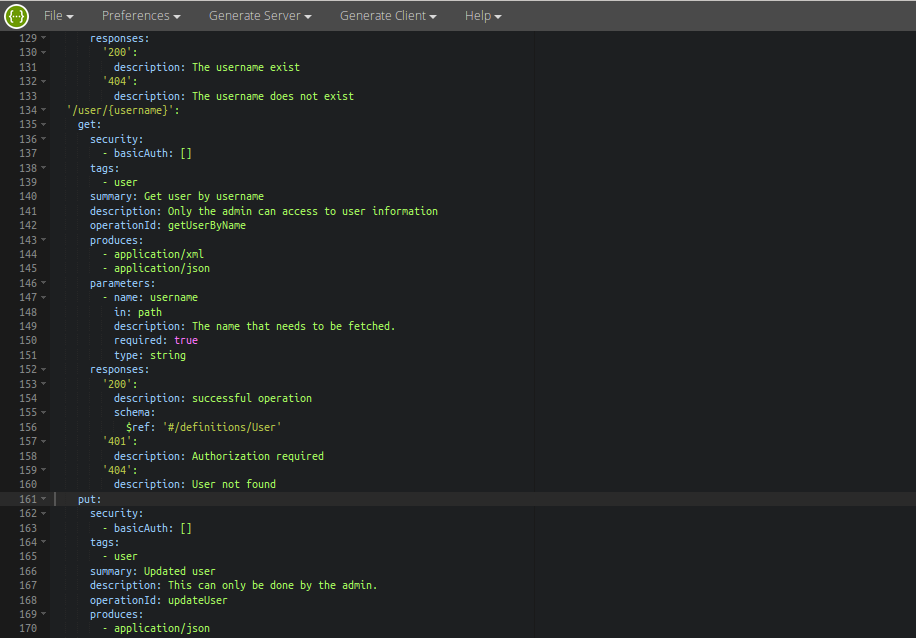
\includegraphics[scale=0.45]{Immagini/swagger-editor.png}
\caption{Swagger editor} 
\end{figure}\\

L'editor permette di descrivere le proprie API tramite un linguaggio chiamato YAML\index{YAML}
che rende la scrittura della documentazione semplice e veloce.
Quello che si ottiene è una documentazione interattiva, con la quale è anche possibili testare le API. 
\begin{figure}[htbp]
\centering
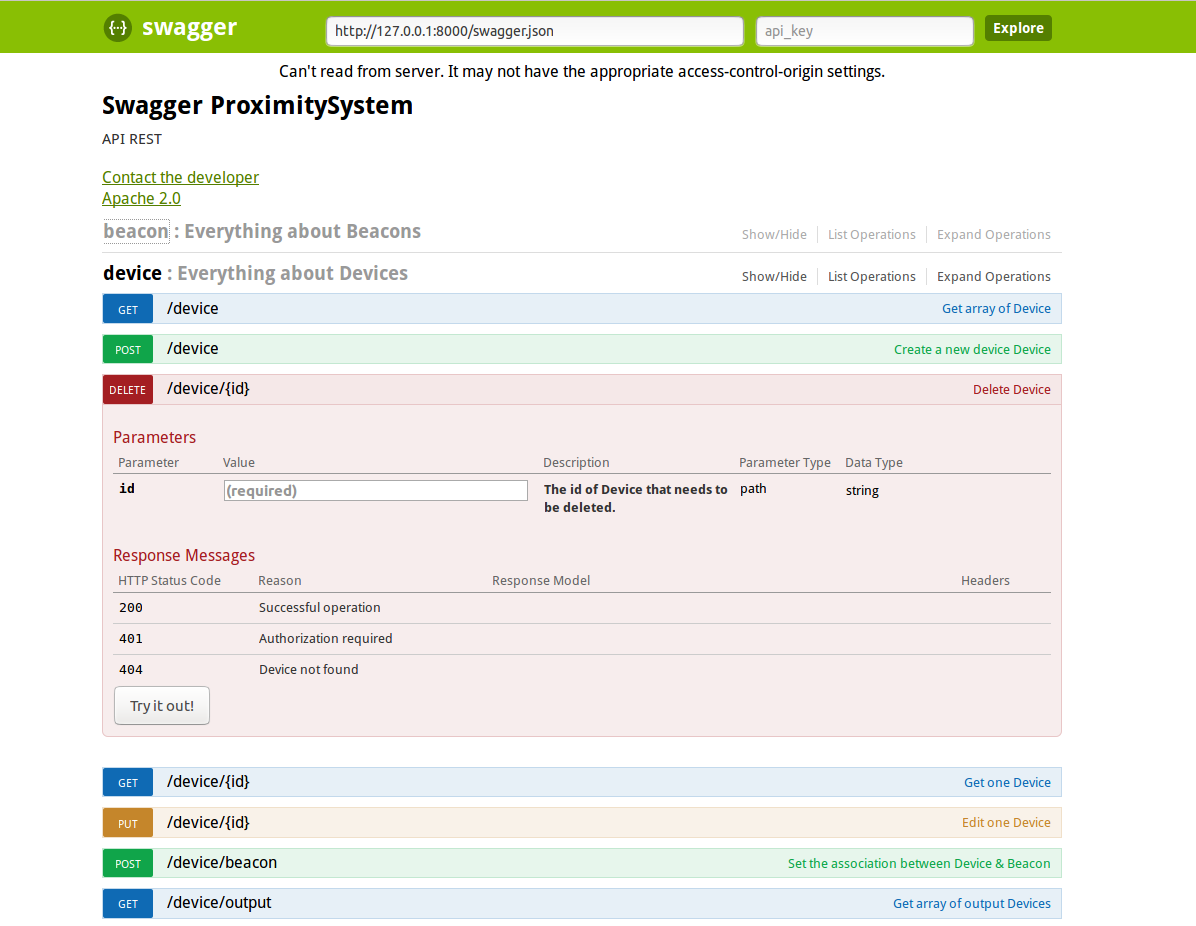
\includegraphics[scale=0.333]{Immagini/swagger-ui.png}
\caption{Swagger ui} 
\end{figure}

\newpage
\section{NodeJS}
Node.js\cite{node} è un interprete javascript per applicazioni di rete lato server. 
È disponibile per diverse piattaforme, come Linux, Microsoft Windows e Apple OS X.
Le applicazioni Node.js vengono costruite utilizzando librerie e moduli che sono disponibili per l'ecosistema ed alcuni di essi li abbiamo utilizzati per la nostra applicazione.
Per iniziare ad utilizzare Node.js, dobbiamo per prima cosa creare un file \texttt{package.json} che descrive la nostra applicazione ed elenchi tutte le sue dipendenze.
NPM (Node.js Package Manager) installa una copia delle librerie in una sotto-cartella chiamata \texttt{node\_modules/}, della cartella principale dell'applicazione. 
Questo comporta diversi benefici, ad esempio isola le diverse versioni delle librerie, evitando così i problemi di compatibilità che si sarebbero avuti se avessimo installato tutto in una cartella standard come \texttt{/usr/lib}.

Il comando \texttt{npm install} creerà la cartella \texttt{node\_modules/}, con dentro tutte le librerie richieste

\begin{lstlisting}[caption={package.json}, style=javaScriptCode][h]
{
  "name": "proximity-system",
  "version": "1.0.0",
  "description": "Backend di Proximity System",
  "scripts": {
    "start": "sudo node server.js",
    "test": "echo \"Error: no test specified\" && exit 1"
  },
  "author": "Marco D'Argenio - Saverio Tosi",
  "license": "Apache 2.0",
  "dependencies": {
    "async": "^2.0.0-rc.6",
    "body-parser": "^1.4.3",
    "cors": "^2.7.1",
    "express": "^4.13.4",
    "frisby": "^0.8.5",
    "mongoose": "^4.5.2",
    "morgan": "^1.7.0",
    "rpi-gpio": "^0.7.0"
  }
}
\end{lstlisting}

Il nome della nostra applicazione è proximity-system. 
La versione è la 1.0.0. 
Sono presenti due script: il primo serve ad avviare il webserver, i permessi di root sono necessari per utilizzare i GPIO nel raspberry; ed un secondo script per eseguire i test. 
Poi sono segnati l'autore, la licenza e l'elenco delle dipendenze. 
I test dell'applicazione li abbiamo scritti con Frisby ed eseguiti con Jasmine-node.

Una libreria particolarmente interessante è async. 
Node.js è stato progettato per essere asincrono.
Qualsiasi operazione che ha a che fare con blocchi di I/O, come leggere un file o interrogare un database, prenderà una callback come ultimo parametro e continuerà l'esecuzione del programma, 
solo quando l'operazione sarà completa il programma richiamerà la callback. 
Ecco un semplice esempio per spiegare meglio il tutto.

\begin{lstlisting}[caption={operazioni asincrone}, style=javaScriptCode, label={lst:async}]
function foo() {
   someAsyncFunction(params, function(err, results) {
      console.log("one");
   });
   console.log("two");
}
\end{lstlisting}

Dal codice \ref{lst:async} ci si potrebbe aspettare che il risultato sia:
\texttt{onetwo}.\\
in realtà potrebbe capitare che l’output sia \texttt{twoone}.
Questa situazione di incertezza dei programmi asincroni viene chiamata esecuzione non deterministica. 
Questo caratteristica permette al programma di essere particolarmente performante, ma ci sono alcuni casi in cui è desiderabile eseguire determinate azioni in un determinato ordine. 

Per questo scopo ci viene incontro Async.
Async è un modulo che fornisce delle funzioni per lavorare con il JavaScript asincrono.
Ce ne sono circa venti tra cui molte classiche come: map, reduce, filter, each, etc. 
Altre più comuni per il controllo del flusso asincrono come parallel e series.
Tutte queste funzioni seguono la convenzione di Node.js di mettere una singola callback come ultimo parametro della funzione. 
L'esempio seguente illustra come stampare i due numeri nell'ordine corretto utilizzando la libreria async:

\begin{lstlisting}[caption={operazioni sincrone}, style=javaScriptCode]
actionArray = [
	function one(cb) {
		someAsyncFunction(params, function(err, results)  {
			if (err) {
				cb(new Error("There was an error"));
			}
			console.log("one");
			cb(null);
		});
	},
	function two(cb) {
		console.log("two");
		cb(null);
	}
]
async.series(actionArray);
\end{lstlisting}

In questo caso siamo sicuri che la prima funzione venga eseguita prima della seconda.

Lo sviluppo del backend, comporta inizialmente l'utilizzo di test. Se pur affrontati in modo superficiale nella nostra applicazione, parleremo dei principali vantaggi che essi comportano:
\begin{itemize}
\item Aiuta lo sviluppatore a capire come verranno consumati i servizi. In modo tale da poterli modificare prima di farli utilizzare ai vari client.
\item Scrivendo i test prima di costruire l'applicazione, il paradigma diventa "rotto/ non implementato finché non passa i test" invece di assumere che funzioni finché qualcosa non va storto.
\end{itemize}

Prima di scrivere il nostro primo test, per iniziare andiamo a definire il file di configurazione.
 
\begin{lstlisting}[caption={test/config/test\_config.js}, style=javaScriptCode]
module.exports = {
	url : 'http://localhost:8000/api/v2.0'
}
\end{lstlisting}

Il nostro server, almeno in fase di sviluppo, sarà eseguito in locale sulla porta 8000. Questo solo per i test iniziale. 
Quando il sistema andrà in produzione e quindi sul RaspberryPi, basterà cambiare questi parametri.

Per preparare i nostri casi di test, per prima cosa ci dobbiamo assicurare di avere un sistema per farli che funzioni correttamente. 
Il seguente codice fa questo per noi

\begin{lstlisting}[caption={test/config/setup\_tests.js - connectDB}, style=javaScriptCode]
function connectDB(callback) {
  mongoClient.connect(dbConfig.testDBURL, function(err, db) {
    assert.equal(null, err);
    proximitysystem_test_db = db;
    console.log("Connesso al server");
    callback(0);
  });
}
\end{lstlisting}

Di seguito, eliminiamo la collection user. 
In questo modo ci assicuriamo di trovarci in uno stato che già conosciamo.

\begin{lstlisting}[caption={test/config/setup\_tests.js - dropUserCollection}, style=javaScriptCode]
function dropUserCollection(callback) {
  console.log("dropUserCollection");
  user = proximitysystem_test_db.collection('User');
  if (undefined != user) {
    user.drop(function(err, reply) {
      console.log('user collection dropped');
      callback(0);
    });
  } else {
    callback(0);
  }
}
\end{lstlisting}

In modo simile eliminiamo poi tutte le altre collection.
Chiudiamo la connessione al database

\begin{lstlisting}[caption={test/config/setup\_tests.js - closeDB}, style=javaScriptCode]
function closeDB(callback) {
  proximitysystem_test_db.close();
}
\end{lstlisting}

Infine, chiamiamo async.series per assicurarci che tutte le funzioni vengano eseguite nell’ordine corretto

\begin{lstlisting}[caption={test/config/setup\_tests.js - async}, style=javaScriptCode]
async.series([
  connectDB,
  dropUserCollection,
  insertAdminInUserCollection,
  dropDeviceCollection,
  dropBeaconCollection,
  dropGPIOCollection,
  insertGPIOInGPIOCollection,
  closeDB]);
\end{lstlisting}

Per i nostri test useremo Frisby.
Frisby è un framework per testare le API REST creato per Node.js e Jasmine che permette di scrivere i test in modo semplice e veloce.
Vediamo qualche esempio:

\begin{lstlisting}[caption={test/user/create\_accounts\_error\_spec.js}, style=javaScriptCode]
TU1_UN = "test6"
TU1_FN = "Test";
TU1_LN = "User10";
TU1_PW = "testUser123";
SP_APP_NAME = 'Proximity System';
\end{lstlisting}

Iniziamo con testare la registrazione. 
In questo caso noi deliberatamente non inseriamo il primo nome, in questo modo ci aspettiamo che il server risponda con uno stato 400 
e una stringa che identifichi il problema.

\begin{lstlisting}[caption={test/user/create\_accounts\_error\_spec.js}, style=javaScriptCode]
frisby.create('POST missing firstName')
    .post(tc.url + '/user',
          { 'lastname' : TU1_LN,
            'username' : TU1_UN,
            'password' : TU1_PW })
    .expectStatus(400)
    .expectHeader('Content-Type', 'application/json; charset=utf-8')
    .expectJSONTypes({'msg' : String})
.toss()
\end{lstlisting}

Adesso, andiamo a vedere alcuni esempi di casi di test che dovrebbero andar a buon fine. per prima cosa definiamo tre utenti.

\begin{lstlisting}[caption={test/user/create\_accounts\_spec.js}, style=javaScriptCode]
TEST_USERS = [{'fn' : 'Test', 'ln' : 'User1',
           	'un' : 'testuser1', 'pwd' : 'testUser123'},
          	{'fn' : 'Test', 'ln' : 'User2',
           	'un' : 'testuser2', 'pwd' : 'testUser123'},
          	{'fn' : 'Test', 'ln' : 'User3',
           	'un' : 'testuser3', 'pwd' : 'testUser123'}]

SP_APP_NAME = 'Reader Test';

var frisby = require('frisby');
var tc = require('./config/test_config');
\end{lstlisting}

In questo caso, stiamo inviando 3 utenti e ci aspettiamo che il server risponda 201 in tutti e tre i casi.

\begin{lstlisting}[caption={test/user/create\_accounts\_spec.js}, style=javaScriptCode]
TEST_USERS.forEach(function createUser(user, index, array) {
    frisby.create('POST user ' + user.un)
        .post(tc.url + '/user',
              { 'firstname' : user.fn,
                'lastname' : user.ln,
                'username' : user.un,
                'password' : user.pwd })
        .expectStatus(201)
        .expectHeader('Content-Type', 'application/json; charset=utf-8')
        .toss()
});
\end{lstlisting}

In questo esempio proviamo a creare un utente con un username già esistente.

\begin{lstlisting}[caption={test/user/create\_accounts\_spec.js}, style=javaScriptCode]
frisby.create('POST duplicate user ')
    .post(tc.url + '/user',
          { 'firstname' : TEST_USERS[0].fn,
            'lastname' : TEST_USERS[0].ln,
            'username' : TEST_USERS[0].un,
            'password' : TEST_USERS[0].pwd })
    .expectStatus(400)
    .expectHeader('Content-Type', 'application/json; charset=utf-8')
.toss()
\end{lstlisting}

Questi test sono stati scritto solo per spiegare il loro funzionamento. 

Prima di iniziare a scrivere le nostre API REST, abbiamo bisogno di definire meglio la configurazione del sistema. 
Per prima cosa, dobbiamo definire come la nostra applicazione si connetterà ad un database. 
Mettendo queste informazioni in un file di configurazione possiamo aggiungere differenti URL dei database a seconda se ci troviamo in fase di sviluppo oppure in produzione.

\begin{lstlisting}[caption={config/db.js}, style=javaScriptCode]
module.exports = {
 	url : 'mongodb://localhost/proximitysystem_test'
}
\end{lstlisting}

\section{Express}
Con express.js\index{Express}, noi abbiamo creato la "applicazione" vera e propria. 
Questa applicazione ascolta in una particolare porta le richieste HTTP in ingresso.
Quando arriva una richiesta, questa passa attraverso una catena di middleware.
Ogni nodo nella catena è definito da un req (request) object e un res (results) object per salvare i risultati. 
Ogni nodo può decidere di eseguire delle operazioni, o di passare i due oggetti al nodo successivo. 
Per aggiungere un nuovo middleware usiamo app.use(). 
Il middleware principale è chiamato “router”, il quale guarda l’URL e il tipo di richiesta per indirizzarlo ad una specifica funzione.

Possiamo finalmente iniziare a scrivere il codice della nostra applicazione, 
che sarà relativamente piccolo in quanto i vari handler saranno in file separati.
\begin{lstlisting}[caption={server.js}, style=javaScriptCode]
var fs = require('fs');
var express = require('express');
var cors = require('cors');
var bodyParser = require('body-parser');
var mongoose = require('mongoose');
var userRoutes = require('./app/routes/user');
var deviceRoutes = require('./app/routes/device');
var beaconRoutes = require('./app/routes/beacon');
var settingRoutes = require('./app/routes/setting');
var gpioRoutes = require('./app/routes/gpio');
var gpio = require('./app/services/gpio');
var db = require('./config/db');
var security = require('./config/security')
var environment = process.env.NODE_ENV;
console.log("Environment: ", environment);
var app = express();
var morgan = require('morgan');
var accessLogStream=fs.createWriteStream(__dirname +'/access.log', {flags: 'a'})
var port = 8000;
mongoose.connect(db.url);
app.use(express.static(__dirname + '/angular'));
app.use(bodyParser.json());
app.use(bodyParser.urlencoded({extended: true}));
app.use(cors());
app.use([userRoutes.authentication,morgan('common',{stream:accessLogStream})]);
userRoutes.addAPIRouter(app);
deviceRoutes.addAPIRouter(app, environment);
beaconRoutes.addAPIRouter(app);
settingRoutes.addAPIRouter(app);
gpioRoutes.addAPIRoutes(app, environment);
\end{lstlisting}

Definiamo il nostro middleware alla fine della catena per la gestione degli URL sbagliati
\begin{lstlisting}[caption={server.js - middleware}, style=javaScriptCode]
app.use(function(req, res, next){
  res.status(404);
  res.json({ error: 'Invalid URL' });
});
// Express route to handle errors
app.use(function (err, req, res, next) {
  if (req.xhr) {
    res.status(500).send('Oops, Something went wrong!');
  } else {
    next(err);
  }
});
\end{lstlisting}

Mettiamo la nostra app in ascolto sulla porta 8000 e gestiamo il segnale SIGINT per interrompere correttamente il webserver

\begin{lstlisting}[caption={server.js - listen}, style=javaScriptCode]
//catches ctrl+c event
process.on('SIGINT', function(){
  console.log("Stop webserver");
  gpio.unexportPins(environment);
});
gpio.init(environment);
app.listen(port);
console.log('GPIO setup completed and server listening on port ' + port);
\end{lstlisting}

\section{Mongoose}
Il passo successivo è quello di modellare i nostri dati con mongoose.
Utilizzeremo mongoose anche per mappare gli oggetti in Node.js nei document in MongoDB\index{MongoDB}\cite{mongodb}.
Le collection da definire sono le seguenti:
\begin{itemize}
\item Beacon
\item Device
\item GPIO
\item User
\end{itemize}

Per questo definiamo uno schema per ciascuna delle 4 collezioni. 
Iniziamo con lo schema degli utenti. 
Notiamo dallo schema, che non solo c'è la tipizzazione dei dati, ma è anche possibile formattare i dati e porre dei vincoli, ad esempio con l'utilizzo di trim.

\begin{lstlisting}[caption={userSchema}, style=javaScriptCode]
var userSchema = new mongoose.Schema({
       block: { type: Boolean, default: false },
       username: { type: String, trim: true, required: true },
       firstname: { type: String, trim: true, required: true },
       lastname: { type: String, trim: true, required: true },
       permission: { type: Number, default: 10},
       created: { type: Date, default: Date.now },
       photo: { type: String, default: "img/account.jpg"},
       password: String,
       theme: { type:String, default: "altTheme"}
    },
    {collection: 'User'}
);
userSchema.index({username : 1}, {unique:true});
var User = mongoose.model('User', userSchema);
\end{lstlisting}

Nel codice dello userSchema, definiamo con mongoose la presenza di un indice. 
Possiamo assicurare che gli indici vengano creati anche se essi non esistono nel nostro database. 
La regola unique assicura che i duplicati non siano permessi. "username: 1" fa in modo che gli username siano mantenuti in ordine crescente.
-1 avrebbe indicato l'ordine decrescente.

Adesso abbiamo bisogno di definire un handler per ogni combinazione di URL/METHOD.
Qui ne descrivo solo uno ma vi ricordo che il resto del codice è disponibile su GitHub
\begin{lstlisting}[caption={get user}, style=javaScriptCode, label={lst:get_user}]
exports.addAPIRouter = function(app, mongoose) {
  	var router = express.Router();
 	router.get('/', function(req, res) {
    if(req.user.block === false && req.user.permission === 0) {
      User.find(function(err, users) {
        if(err) {
          res.status(500).send({msg: err.errmsg});
        } else if(users && users.length>0) {
          res.status(200).send(users);
        } else {
          res.status(200).send([]);
        }
      });
    } else {
      res.status(401).send({msg: 'Authorization required'})
    }
 });
\end{lstlisting}


I principali metodi messi a disposizione dall'oggetto mongoose.
Schema sono find, save, findAndRemove e update. 
Nel codice \ref{lst:get_user} vediamo come sia semplice accedere all'elenco degli utenti. 
Basta infatti richiamare User.find().
\chapter{Websocket}
\label{chap:websocket}
\nocite{html5}
Nel capitolo \ref{chap:scelta} abbiamo parlato di come e con quali tecnologie sono state implementate le API REST di proximity system.  
Queste API danno la possibilità a chiunque di implementare un proprio client per qualsiasi dispositivo. 
Il problema di questi servizi è che che sono di tipo pull, ovvero dev'essere il client a chiedere informazioni al server. 
Il server non può inviare i dati aggiornati appena sono disponibili,
ma soltanto quando un client li richiede.

In questo capitolo andremo a vedere come risolvere questo problema con il metodo di comunicazione più potente introdotto con la specifica HTML5: le WebSocket.
Queste non sono altro che un canale di comunicazione full-duplex operante su una singola socket che permette di migliorare drasticamente sia la quantità di traffico che la latenza di tutte le applicazione web basate sulla visualizzazione di dati in tempo reale e sugli eventi.
  
\section{Panoramica della applicazione real-time e HTTP}
\label{sec:real-time}
Prima di andare nel dettaglio nella specifica WebSocket, vediamo quali sono e come funzionano i principali "hack" utilizzati per simulare un'applicazione real-time con il protocollo HTTP.

Nei tradizionali siti web quando un server HTTP riceve la richiesta, il server genera la pagina richiesta personalizzata per il client, la inoltra ed è il client che poi fa il render della risposta e la visualizza a video.
Esistono molti casi, come la disponibilità di biglietti per un evento, dati azionari etc. in cui i dati inviati dal server potrebbero già essere deprecati nel momento in cui il client fa il render della pagina. 
Per avere gli ultimi dati, bisogna aggiornarli continuamente, ad esempio manualmente, anche se ovviamente non rappresenta una soluzione ottimale.

Comet\index{Comet} è un modello per le web application nel quale una particolare gestione 
delle richieste HTTP permette al web server di inviare notifiche push al browser, senza che il browser faccia una richiesta specifica.
Esistono diverse tecniche che permettono di implementare questo modello basato sugli eventi. 

La più diffusa tra le tecniche comet è il polling, che consiste nell'invio di richieste HTTP a intervalli regolari con una risposta immediata da parte del server. 
Questa tecnica è efficiente nei casi in cui si conosce a prescindere ogni quanto tempo i dati verranno aggiornati dal server.
Come è facile immaginare non è sempre semplice prevedere con quale cadenza i dati verranno aggiornati, causando un numero elevato di richieste non necessarie.
Quello che ne deriva è l'apertura e la chiusura di un alto numero di connessioni e quindi l'utilizzo di risorse non strettamente necessarie.

Una possibile soluzione è l'implementazione del long-polling, dove il client invia una richiesta al server che risponderà soltanto se i dati sono stati aggiornati e farà scadere la richiesta altrimenti. È importante far notare che se il numero di aggiornamenti è alto, non si hanno vantaggi rispetto al polling tradizionale.
Quello in Figura \ref{fig:timing} è un esempio di long-polling in azione preso da messenger. 

\begin{figure}[htpb!]
  \centering
  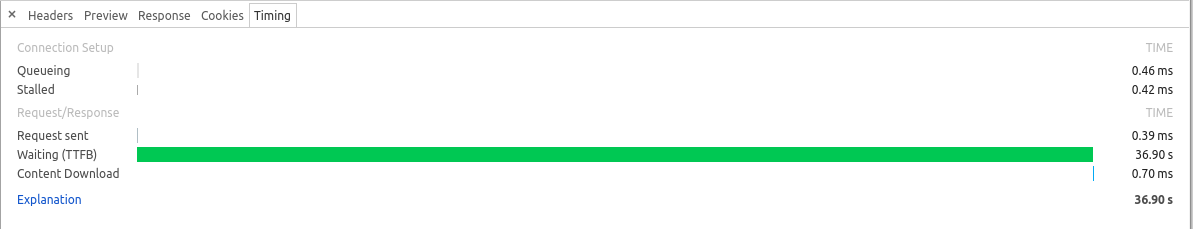
\includegraphics[width=1\textwidth]{timing}
  \caption{Esempio di long-polling}
  \label{fig:timing}
\end{figure}

Un'altra tecnica, che prende il nome di streaming, consiste in una connessione completa tra client e server, in cui il server mantiene la connessione aperta con un aggiornamento costante delle informazioni per un tempo indeterminato, per poi aggiornare la risposta con l'arrivo di nuovi dati, sempre mantenendo aperta la connessione.

In questo modo la connessione rimane aperta per i messaggi seguenti.
Il problema è dato dal fatto che lo streaming è incapsulato in una richiesta HTTP e in quanto tale un eventuale firewall o proxy nel mezzo potrebbero interferire bufferizzando la risposta.
Per questo motivo molti sistemi passano automaticamente al long-polling se rilevano la presenza di qualche proxy.
Una possibile soluzione alternativa è quella di utilizzare connessioni TLS per impedire il buffering della risposta,
ma in questo caso bisogna prendere in considerazione l'utilizzo di
maggiori risorse da parte del server.

Tutte le tecniche sopra descritte hanno in comune due problemi:
\begin{itemize}
\item prevedono l'utilizzo dell'header HTTP
\item prevedono l'invio di messaggi solo dal server al client
\end{itemize}
Il primo problema consiste nel fatto che l'header HTTP contiene molte informazioni inutili al fine della comunicazione stessa, occupando banda e aumentando la latenza della connessione.

Il secondo consiste nel fatto in cui se l'utente ha la necessita di inviare dati al server, 
dovrà instaurare una nuova connessione per poterlo fare.
Ciò comporta tutta una serie di problematiche per mantenere i dati
sincronizzati tra tutte le connessione.

In altre parole, il protocollo HTTP 1.1 è un protocollo pull e non push.
In quanto tale, realizzare una webapp con il modello publish/subscribe attraverso comunicazioni HTTP half-duplex è più complicato di quanto sembri, sopratutto per soluzioni scalabili.

\section{Introduzione alle WebSocket}
Ian Hickson, uno dei principali responsabili della specifica HTML5, inizialmente definì le WebSocket nella sezione specifica dedicata ai metodi di comunicazione con il nome di "TCPConnection".
Questa specifica si è evoluta poi a tal punto da far definire le WebSocket in una specifica indipendente come la geolocalizzazione, i Web Worker etc. per mantenere la discussione focalizzata.

Il protocollo WebSocket viene descritto nel RFC 6455\cite{RFC6455} ed è diviso in due parti: una che descrive l'handshake e una per il trasferimento dei dati.

Una volta che il client e il server hanno completato l'handshake, se è andato a buon fine, allora i due possono iniziare a comunicare.
Quello che si crea è un canale di comunicazione full-duplex dove sia il client che il server, indipendentemente l'uno dall'altro, possono inviare dei dati.

Dopo l'handshake, i dati che vengono scambiati prendono il nome di "messaggi". 
A livello fisico, un messaggio è composto da uno o più frame.
Quindi un messaggio WebSocket non corrisponde necessariamente ad un particolare frame, in quanto il messaggio può essere frammentato e poi ricomposto da qualsiasi intermediario tra le due parti.

Un frame ha associato un determinato tipo. 
Ogni frame dello stesso messaggio contiene lo stesso tipo di dati.
Possiamo identificare dei dati di tipo testo(UTF-8), dati binari e frame di controllo.
La versione corrente del protocollo definisce sei tipi di frame e ne lascia altri dieci per future implementazioni.
\subsection{L'handshake WebSocket}
\label{sec:handshake}
L'handshake è stato progettato per essere compatibile con i server basati sul protocollo HTTP, in modo tale che una singola porta possa essere utilizzata sia dai client che vogliono comunicare con il WebServer sia dai client WebSocket.
Per questo motivo l'handshake è una richiesta di HTTP upgrade.
\begin{lstlisting}[caption={client handshake}, style=javaScriptCode]
	GET /chat HTTP/1.1
	Host: server.example.com
	Upgrade: websocket
	Connection: Upgrade
	Sec-WebSocket-Key: dGhlIHNhbXBsZSBub25jZQ==
	Origin: http://example.com
	Sec-WebSocket-Protocol: chat, superchat
	Sec-WebSocket-Version: 13
\end{lstlisting} 

Come stabilito nel RFC 2616\cite{RFC2616}, i campi dell'header possono essere inviati in qualsiasi ordine.  
Il metodo GET viene utilizzato sia per identificare la WebSocket corretta, sia per far in modo che domini multipli possano essere serviti da un singolo indirizzo IP e per permettere la gestione di più WebSocket in un singolo server.

Il client include nell'header il nome dell'host del server così come descritto in RFC2616, in modo tale che sia il client che il server
possano verificare che l'host in uso sia quello corretto.

Campi dell'header addizionali possono essere aggiunti  per selezionare
delle opzioni del protocollo WebSocket.
Le opzioni tipiche che vengono utilizzate sono:
\begin{itemize}
\item \textbf{Sec-WebSocket-Protocol}: lista dei sotto protocolli disponibili nel client;
\item \textbf{Sec-WebSocket-Extension}: lista delle estensioni disponibili nel client;
\item \textbf{Origin}: per la gestione del CORS.
\end{itemize}

Il campo \emph{Origin} vieni utilizzato come contromisura per 
l'utilizzo non autorizzato del server WebSocket da script eseguiti nel browser.
Se il server non vuole accettare una connessione da una determinata origine, 
può scegliere di rifiutare la connessione inviando un codice di errore HTTP appropriato.
Questo campo ha senso solo per i client che sono browser, in quanto tutti gli altri possono modificarlo a loro piacimento.

Adesso, il server deve dimostrare al client che ha ricevuto un messaggio di handshake e deve stare attento a non accettare richieste che non siano per le WebSocket.
In modo tale da prevenire eventuali attacchi generati con un XMLHttpRequest o l'invio di dati da un form.

Per dimostrare che ha ricevuto l'handshake corretto, il server deve prendere due dati e metterli insieme per generare una risposta.
Il primo dato viene preso dal campo \emph{Sec-WebSocket-Key}.
il secondo è la stringa che rappresenta il GUID(Globally Unique Identifier RFC4122\cite{RFC4122}) "258EAFA5-E914-47DA-95CA-C5AB0DC85B11".
Ad esempio, se prendiamo i dati dal handshake precedente, 
il server deve concatenare il GUID e il \emph{Sec-WebSocket-Key} ottenendo la stringa "dGhlIHNhbXBsZSBub25jZQ==258EAFA5-E914-47DA-95CA-C5AB0DC85B11".
Poi il server deve prendere l'hash SHA-1 di questa stringa, ovvero 
0xb3 0x7a 0x4f 0x2c 0xc0 0x62 0x4f 0x16 0x90 0xf6 0x46 0x06 0xcf 0x38 0x59 0x45 0xb2 0xbe 0xc4 0xea.
Questo valore deve essere poi codificato in base64, 
ottenendo "s3pPLMBiTxaQ9kYGzzhZRbK+xOo=".
Questo valore dovrà essere inserito nell'header nel campo Sec-WebSocket-Accept".

L'handshake del server è molto più semplice rispetto a quello del client.

\begin{lstlisting}[caption={server handshake}, style=javaScriptCode]
	HTTP/1.1 101 Switching Protocols
	Upgrade: websocket
	Connection: Upgrade
	Sec-WebSocket-Accept: s3pPLMBiTxaQ9kYGzzhZRbK+xOo=
\end{lstlisting} 
\label{sec:serv_handshake}

Se il valore di Sec-WebSocket-Accept non è quello aspettato, se manca qualche header, o se lo stato HTTP è diverso da 101, la connessione non verrà stabilita e i frame WebSocket non verranno inviati.
L'header può anche includere i campi delle opzioni e settera eventuale cookie.
 
\subsection{L'interfaccia}
Utilizzare le WebSocket in un'applicazione JavaScript è molto semplice.
Per la connessione con l'host remoto è sufficiente creare una nuova istanza WebSocket, fornendo al nuovo oggetto l'URL con il quale si desidera aprire la connessione.
I prefissi \texttt{ws://} e \texttt{wss://} indicano rispettivamente una connessione WebSocket e una connessione WebSocket sicura.
La connessione WebSocket è stabilita passando dal protocollo HTTP a quello WebSocket, durante l'handshake iniziale tra client e server, attraverso la stessa connessione TCP/IP. Dopo aver stabilito la connessione i frame di dati WebSocket possono essere inviati e ricevuti in modalità full-duplex.
La connessione stessa è esposta tramite l'evento \texttt{message} e il metodo \texttt{send} definiti nell'interfaccia WebSocket.
Scrivendo il codice è possibile utilizzare dei \emph{listener} asincroni per gestire ogni fase del ciclo di connesione.
\begin{lstlisting}[caption={interfaccia WebSocket}, style=javaScriptCode]
url = "ws://example.com/echo";
socket = new WebSocket(url);
socket.onopen = function() {
	console.log("WebSocket aperta");
	socket.send("Grazie per aver accettato questa WebSocket");
}
socket.onmessage = function(e) {
	console.log(e.data);
}	
socket.onclose = function(e) {
	console.log("connessione chiusa");
}
\end{lstlisting} 
\label{sec:interfaccia_websocket}
\subsection{Aumento delle prestazioni}
Le WebSocket HTML offrono vantaggi tali da spingere Ian Hickson (Google) a dichiarare: \\
\textit{"Reducing kilobytes of data to 2 bytes is more than "a little more byte efficient", 
and reducing latency from 150ms (TCP round trip to set up the 
connection plus a packet for the message) to 50ms (just the packet for the 
message) is far more than marginal. 
In fact, these two factors alone are enough to make WebSocket seriously interesting to Google."}\footnote{\url{www.ietf.org/mail-archive/web/hybi/current/msg00784.html}}
  
Per illustrare quanto possono essere efficienti le WebSocket,
andremo a confrontare il traffico e la latenza di un'applicazione web prima implementata tramite polling e poi tramite WebSocket.

Dato che il miglioramento delle performance in Proximity System è minimo, 
prenderemo in considerazione un'ipotetica applicazione che visualizza dati in tempo reale i dati di una macchina da corsa: velocità; giri del motore; tempo del giro, posizione, km percorsi.
Supponiamo che le 2 nostre applicazioni, quella basata sul polling e qualle basata sulle WebSocket, ricevano i dati tramite il seguente JSON:
\begin{lstlisting}[caption={JSON dati macchina}, style=javaScriptCode]
{
	"lap_time": "35.256", 
	"speed": "124",
	"gear": "4",
	"RPM": "15600",
	"mileage": "12563.02"
}
\end{lstlisting} 

In questo caso la quantità di dati che il server invia al client è pari al numero di caratteri presenti nel JSON, escludendo gli spazi, le tabulazioni e i ritorni a capo che si possono omettere contiamo 81 caratteri e quindi 81 byte di dati.
Il problema è che oltre agli 81 byte dei dati effettivi, ogni richiesta XMLHttpRequest deve considerare sia l'header inviato dal client che quello inviato dal server in risposta.
Giusto per far un esempio, osserviamo i due header di una richiesta fatta utilizzando ProximitySystem
\begin{lstlisting}[caption={header client}, style=javaScriptCode]
GET /api/v2.0/gpio HTTP/1.1\r\n
Host: localhost:8000
Connection: keep-alive
Cache-Control: max-age=0
Accept: application/json, text/plain, */*
If-Non-Match: If-None-Match: W/"4dc-Uz68k8B/IopHdTlOHcquQA"
User-Agent: Mozilla/5.0 (X11; Linux x86_64) AppleWebKit/537.36 (KHTML, like Gecko) 
				Chrome/52.0.2743.116 Safari/537.36
Authorization: Basic YWRtaW46MTIzNDU2
DNT: 1
Referer: http://localhost:8000/
Accept-Encoding: gzip, deflate, sdhc
Accept-Language: it-IT,it;q=0.8,en-US;q=0.6,en;q=0.4
\end{lstlisting}
Solo nell'header di richiesta ci sono 484 caratteri
\begin{lstlisting}[caption={header server}, style=javaScriptCode]
HTTP/1.1 200 OK
X-Powered-By: Express
Content-Type: application/json; charset=utf-8
Content-Length: 1246
Etag: W/"4de-K40aEhIMswWt/3FPFcGKCQ"
Date: Mon, 29 Aug 2016 15:05:16 GMT
Connection: keep-alive

\end{lstlisting} 
Aggiungendo i 210 della risposta otteniamo 694 byte di dati non necessari per ogni richiesta. 
È vero che questo è solo un esempio, e ci saranno situazioni con meno dati nell'header, ma è bene sapere che in alcuni casi le informazioni nell'header possono arrivare vino a 2000 byte.
Andando a ricapitolare possiamo vedere come il rapporto tra dati inutili(694 byte) e dati utili(81 byte) sia di  circa 8:1, un gran spreco di dati.
Vediamo cosa accadrebbe distribuendo questa applicazione ad un ampio numero di utenti. 
ipotizziamo tre scenari di utilizzo:
\begin{enumerate}
\item 1.000 client che eseguono il polling ogni secondo.
il traffico equivale a: 694 x 1.000 = 694.000 byte = 5.552.000 bit al secondo = 5,2 Mbps;
\item 10.000 client che eseguono il polling ogni secondo.
il traffico equivale a: 694 x 10.000 = 6.940.000 byte = 55.520.000 bit al secondo = 52 Mbps;
\item 100.000 client che eseguono il polling ogni secondo.
il traffico equivale a: 694 x 100.000 = 69.400.000 byte = 555.200.000 bit al secondo = 529 Mbps.
\end{enumerate}
Adesso che abbiamo visto la quantità di banda che si spreca utilizzando il polling, 
andiamo ad analizzare come si comporta la stessa applicazione con l'utilizzo delle WebSocket.
\begin{figure}[htpb!]
  \centering
  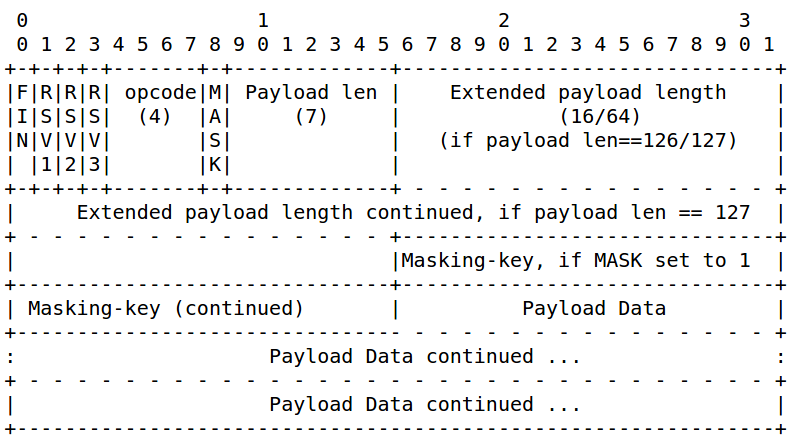
\includegraphics[width=1\textwidth]{frame}
  \caption{Frame WebSocket}
  \label{fig:frame}
\end{figure}
Osservando il frame si può evincere che le informazioni non necessarie possono variare da un minimo di 2 byte ad un massimo di 16 byte.
Ecco lo scenario del traffico prendendo in considerazione il caso peggiore:
\begin{enumerate}
\item 1.000 client che ricevono un messaggio al secondo.
il traffico equivale a: 16 x 1.000 = 16.000 byte = 128.000 bit al secondo = 0,12 Mbps;
\item 10.000 client che ricevono un messaggio al secondo.
il traffico equivale a: 16 x 10.000 = 160.000 byte = 1.280.000 bit al secondo = 1,22 Mbps;
\item 100.000  client che ricevono un messaggio al secondo.
il traffico equivale a: 16 x 100.000 = 1.600.000 byte = 12.800.000 bit al secondo = 12,20 Mbps.
\end{enumerate}
\begin{figure}[htpb!]
  \centering
  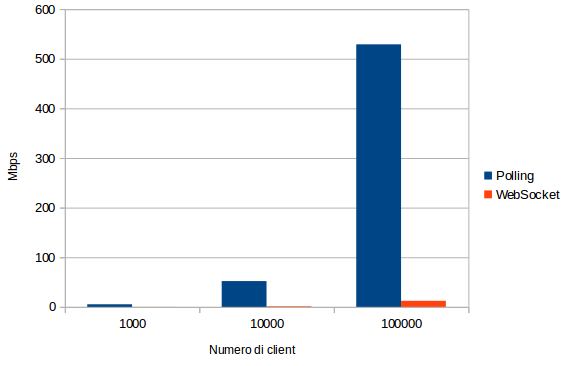
\includegraphics[width=0.8\textwidth]{dati_non_necessari}
  \caption{Traffico dati non necessario}
  \label{fig:traffico}
\end{figure}
Basta guardare la Figura \ref{fig:traffico} per rendersi conto dell'inutile mole di dati che viene generata se si realizza un'applicazione real-time con il polling.

Per quanto riguarda la latenza, l'aumento delle performance è illustrate in Figura \ref{fig:latenza}.
Se ipotizziamo che un pacchetto per arrivare dal browser al server impieghi 50 ms, l'applicazione con il polling genera molta latenza in più rispetto a quella implementata tramite WebSocket, 
perché per ogni risposta completa deve essere inviata una nuova richiesta.    
\begin{figure}[htpb!]
  \centering
  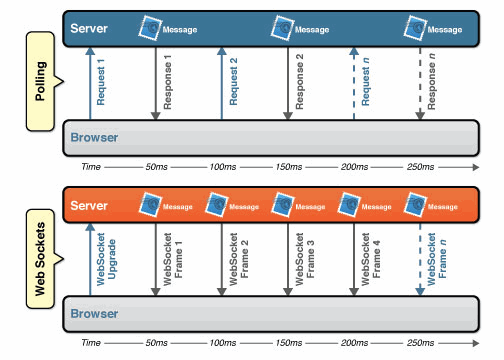
\includegraphics[width=0.8\textwidth]{latenza}
  \caption{Latenza}
  \label{fig:latenza}
\end{figure}
\subsection{Supporto dei browser}
La specifica WebSocket ormai ha qualche anno, per la precisione, la versione standard definita nel RFC6455 è di dicembre 2011.
Nonostante ciò, le WebSocket sono supportate solo nei browser più recenti.
\begin{table}[htbp]
\begin{center}
\begin{tabular}{|l|l|l|l|l|l|}
\hline
Versione & Chrome & Firefox & Internet Explorer & Opera & Safari \\
\hline
76 & 6 & 4.0 & No & 11.00(disabilitato) & 5.0.1\\
\hline
7 & No & 6.0 & No & No & No \\
\hline
10 & 14 & 7.0 & HTML5 Labs & ? & ?\\
\hline
RFC 6455 & 16 & 11.0 & 10 & 12.10 & 6.0\\
\hline
\end{tabular}
\end{center}
\caption{Supporto dei browser}
\label{tab:browser}
\end{table}

\begin{table}[htbp]
\begin{center}
\begin{tabular}{|l|l|l|l|l|l|}
\hline
Versione & Android & Firefox Mob. & IE Mob. & Opera Mob. & Safari Mob.\\
\hline
76 & ? & ? & ? & ? & ?\\
\hline
7 & ? & ? & ? & ? & ? \\
\hline
10 & ? & 7.0 & ? & ? & ?\\
\hline
RFC 6455 & 16(Chrome) & 11.0 & ? & 12.10 & 6.0\\
\hline
\end{tabular}
\end{center}
\caption{Supporto dei browser Mobile}
\label{tab:mobile}
\end{table}
Nelle Tabelle \ref{tab:browser} e \ref{tab:mobile} è possibile vedere, rispettivamente per desktop e per mobile, il supporto dei vari browser per le diverse specifiche delle WebSocket.

Quando si crea una WebApp con le WebSocket è importante prendere in considerazione anche la possibilità che esse non siano supportate dal client e quindi implementare anche una soluzione alternativa, per l'appunto, nel caso non sia possibile utilizzare le WebSocket.
Esistono diversi framework che forniscono supporto completo sia per l'implementazione del client che del server che risolvono tutti i problemi di compatibilità che potrebbero presentarsi.
Tra i framework più popolari troviamo:
\begin{itemize}
\item Kaazing;
\item LightStreamer; 
\item Socket.io.
\end{itemize}
Nel paragrafo successivo vedremo in dettaglio come implementare sia il client ed il server di un'applicazione real-time con Socket.io

\section{Socket.io}
\label{sec:socket.io}
Socket.io permette di sviluppare applicazione client-server real-time, 
senza doversi preoccupare delle problematiche relative alle WebSocket.
Ad esempio, se un client non supporta le WebSocket, socket.io implementerà lo stesso servizio con il polling, il tutto in maniera trasparente al programmatore.

In questa sezione scriveremo il codice di una chat, lo stesso proposto nel sito di Socket.io ma utilizzando Angular nel client, 
per farne vedere sia l'utilizzo lato frontend che backend.

\subsection{Backend}
Le uniche dipendenze di cui ha bisogno il nostro backend sono: express e socket.io.
Il codice è molto semplice e non ha bisogno di particolari spiegazioni.
Il server è in ascolto sulla porta 3000 sia di connessioni HTTP sia WebSocket.
Se riceve una richiesta http risponderà con la WebApp in Angular,
altrimenti, gestirà la WebSocket.
\begin{lstlisting}[caption={backend chat socket.io}, style=javaScriptCode]
var express = require('express');

var app = express();
var http = require('http').Server(app);
var io = require('socket.io')(http);
var port = 3000;

app.use(express.static(__dirname + '/angular'));

io.on('connection', function(socket){
  console.log('a user connected');

  socket.on('disconnect', function(){
    console.log('user disconnected');
  });

  socket.on('chat message', function(msg){
    console.log('message: ' + msg);
    io.emit('chat message', msg);
  });
});

http.listen(port, function(){
  console.log("Server listening on port " + port);
});
\end{lstlisting} 
L'unica cosa che fa il server è inviare in broadcast a tutte le socket connesse i messaggi che riceve dalle singoli connessioni.
Se non avessimo utilizzato Socket.io avremmo dovuto implementare soluzioni alternative nel caso in cui le WebSocket non fossero disponibili nel client o 
l'handshake non andasse a buon fine, in questo caso, invece, è Socket.io che si occupa di gestire tutti i possibili problemi e fornire una soluzione equivalente, in maniera sempre trasparente al programmatore.
\subsection{Frontend}
Il frontend, molto semplicemente, invierà i messaggi scritti dall'utente tramite Socket.io al server e visualizzerà a video i messaggi ricevuti, il tutto, real-time.
Per utilizzare Socket.io come se fosse un servizio di Angular, 
abbiamo installato il plugin \texttt{angular-socket-io}, disponibile tramite bower e inizializzato come segue.
\begin{lstlisting}[caption={service mySocket}, style=javaScriptCode]
angular.module('socketApp.services.socket',[])
.factory('mySocket', function(socketFactory) {
  var myIoSocket = io.connect();

    mySocket = socketFactory({
      ioSocket: myIoSocket
    });

  return mySocket;
});
\end{lstlisting} 
A livello di controller basta iniettare il servizio come dipendenza e si
possono utilizzare i listener e i metodi messi a disposizione da Socket.io.
Nel codice che segue semplicemente se arriva un nuovo messaggio viene aggiunto all'array di messaggi.
\begin{lstlisting}[caption={controller mySocket}, style=javaScriptCode]
angular.module('socketApp.controllers.home', [])
.controller('HomeCtrl',  function($scope, mySocket) {
  $scope.messages = [];
  $scope.message = "Scrivi qualcosa";

  mySocket.on('chat message', function(data) {
    $scope.messages.push({text: data});
  })

  $scope.send = function() {
    mySocket.emit('chat message', $scope.message);
    $scope.message = "";
  };
});
\end{lstlisting} 
Questo è tutto, il codice completo dell'esempio è disponibile sul mio GitHub\footnote{\url{https://github.com/save91/angular-chat-socket.io}}.




\chapter{Implementazione}
In questo capitolo mostreremo come sono stati implementati i servizi REST per i requisiti funzionali elencati nella tabella \ref{tab:req:fun}.
Vedremo quindi per ogni requisito quali API sono state create, come sono state documentate ed il codice che abbiamo implementato per ciascuna di esse.

\section{FUN-01}
Per implementare il primo requisito funzionale che prevede l'utilizzo dei propri dispositivi con l'app, abbiamo creato quattro servizi.
Il primo, /device/output/, serve per richiedere l'array dei propri dispositivi.
Qui di seguito il codice relativo alla rotta:
\begin{lstlisting}[caption={/webserver/app/routes/device.js output}, style=javaScriptCode]
  router.get('/output', function(req, res) {
    if(req.user.block) {
      res.status(401).send({'msg':'Authentication required'});
    } else {
      Device.find({_GPIO:{$ne: null}, permission:{$gte: req.user.permission}, 
                                                      io:"output"})
        .populate('_Beacon _GPIO')
        .exec(function (err, devices) {
          if(err) {
            debugger;
            res.status(500).send({msg: err.errmsg});
          } else if(devices && devices.length>0) {
            res.status(200).send(devices);
          } else {
            res.status(200).send([]);
          }
      });
    }
  });
\end{lstlisting}
Il server controlla se l'utente che ha richiesto la lista dei dispositivi abbia effettuato il login e non sia stato bloccato.
Se l'utente non ha i permessi il server risponderà con un 401, altrimenti ricercherà tra tutti i dispositivi quelli che hanno un GPIO configurato e a cui può accedere l'utente. 
Così come descritto nella figura \ref{fig:device:output}\footnote{La documentazione è state scritta con swagger. Per consultarla, una volta avviato il backend, basta visitare la pagina \url{http://localhost:8000/swagger-ui/dist/} }. 

\begin{figure}[h]
\centering
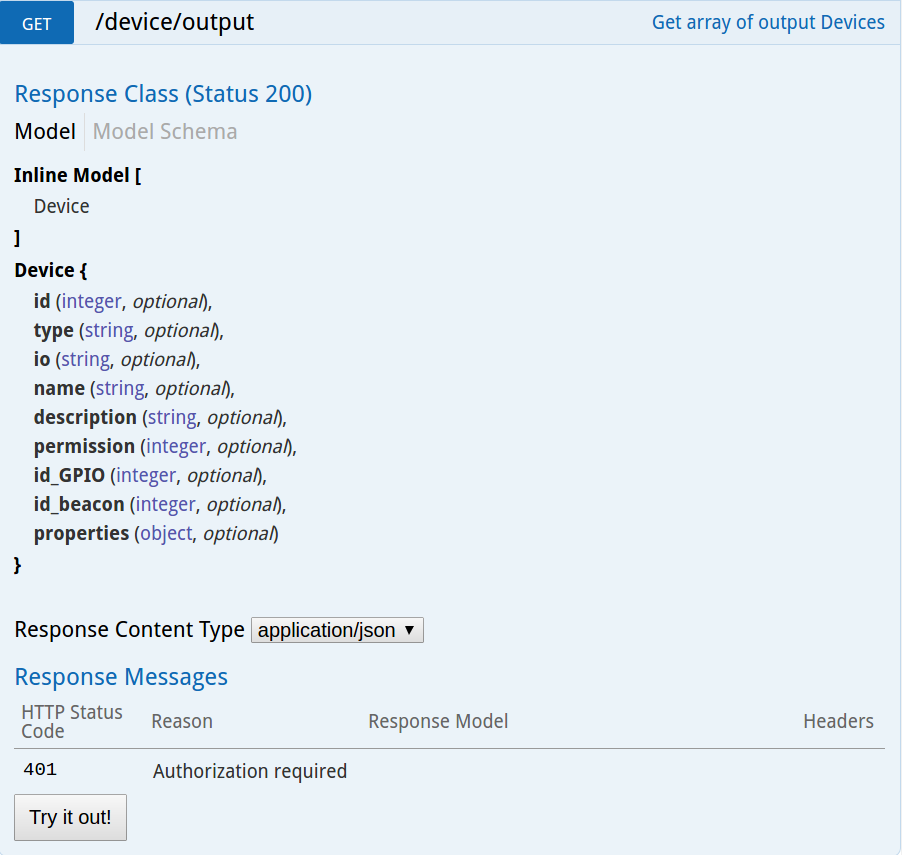
\includegraphics[width=1\textwidth]{API/device_output.png} 
\caption{Documentazione /device/output}
\label{fig:device:output}
\end{figure}

Le altre tre sono /device/on, /device/off e /device/push.
Queste permettono di gestire i GPIO associati ai dispositivi settandoli rispettivamente a true, false e di inviare un impulso.

\newpage
Per queste tre rotte vedremo il codice solo della prima perché sono molto simili tra loro.
\begin{lstlisting}[caption={/webserver/app/routes/device.js on}, style=javaScriptCode]
  //need permission to do an action
  router.put('/:id/on', function(req, res) {
    if(req.user.block) {
      res.status(401).send({'msg':'Authentication required'});
    } else {
      Device.findById(req.params.id)
        .populate('_GPIO')
        .exec(function(err, device) {
          if(err) {
            debugger;
            res.status(500).send({msg: err.errmsg});
          } else if(device) {
            GPIO.update({_id: device._GPIO}, {value: true}, {}, 
                                         function (err, ok) {
              if(err) {
                res.status(500).send({msg: err.errmsg});
              } else {
                pin.setPin(device._GPIO.GPIO, true, function(err) {
                  if (err) {
                    res.status(500).send('Oops, Something went wrong! '
                                                      + err);
                  } else {
                    io.emit('update:device');
                    io.emit('update:gpio');
                    res.status(200).send({'msg':'ok'});
                  }
                }, environment);
              }
            });
          } else {
            res.status(404).send([]);
          }
        });
      }
    });
\end{lstlisting}
Quello che salta all'occhio sono le due funzioni pin.setPin e io.emit.
La funzione pin.setPin permette di settare il GPIO del RaspberryPI.
Mentre io.emit serve per inviare una notifica push a tutti i client connessi che li avvisa che i dati dei dispositivi e dei GPIO sono stati aggiornati, saranno poi i client a decidere se è il caso di aggiornarli oppure no.  

Come passare i parametri al server e le possibili risposte sono descritte nella documentazione.
\begin{figure}[h]
\centering
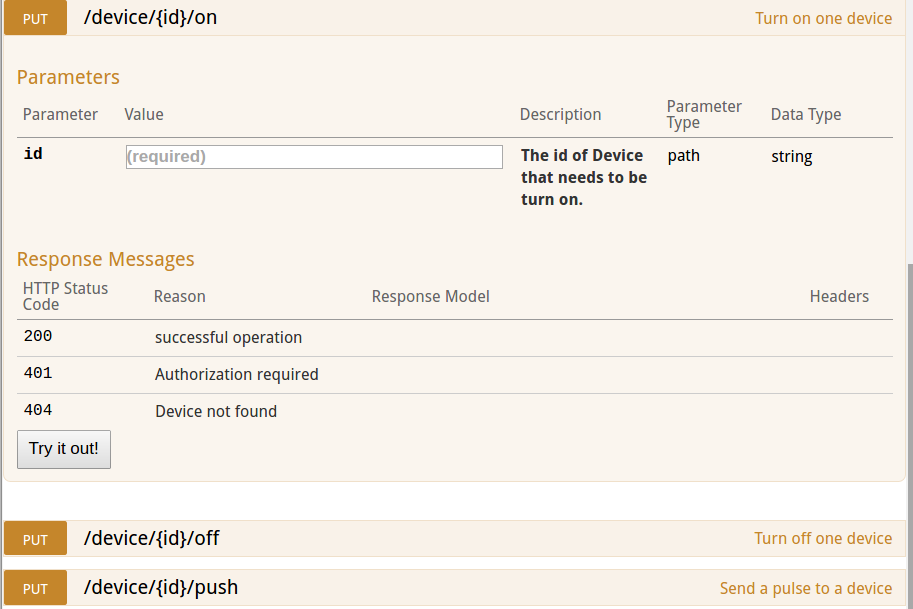
\includegraphics[width=1\textwidth]{API/device_on.png} 
\caption{Documentazione /device/{id}/on}
\label{fig:device:on}
\end{figure}

Nella figura \ref{fig:device:on} si vedono solamente i parametri e i messaggi di risposta della prima rotta, ma sono gli stessi anche per le altre due.

\section{FUN-02}
Il secondo requisito parla di fornire agli utenti dell'app la possibilità di effettuare il login e la registrazione.
Lato backend si è tradotto in tre API.
Una richiesta in post per il login.
Una richiesta in post per la registrazione e un'ultima richiesta per verificare se l'username scelto dall'utente è disponibile in quanto deve essere univoco. 

\begin{lstlisting}[caption={/webserver/app/routes/user.js login}, style=javaScriptCode]
  router.post('/login', function(req, res) {
    if(req.body.username && req.body.password) {
      User.findOne({
        'username': req.body.username,
        'password': req.body.password
      }, 'block username firstname lastname permission photo
       theme',function(err, user) {
        if(err) {
          res.status(500).send({'msg': err});
        } else if(user) {
          res.status(200).send(user);
        } else {
          res.status(400).send({'msg': 'Fail'});
        }
      });
    } else {
      res.status(400).send({'msg': 'Fail'});
    }
  });
  
  router.post('/', function(req, res) {
    if(req.body.firstname && req.body.lastname && 
                  req.body.username && req.body.password) {
      var newUser = new User({
        firstname: req.body.firstname,
        lastname: req.body.lastname,
        username: req.body.username,
        password: req.body.password,
        photo: req.body.photo,
        block: true
      });
      newUser.save(function (err) {
        if(err) {
          debugger;
          if(err.code === 11000) {
            res.status(400).send({msg: "duplicate username"});
          } else {
            res.status(500).send({msg: err.errmsg});
          }
        } else {
          io.emit('update:user');
          res.status(201).send(newUser);
        }
      });
    } else {
      res.status(400).send({'msg': 'missing data'})
    }
  });

  router.post('/check_username', function(req, res) {
    User.findOne({
      'username': req.body.username,
    }, function(err, user) {
      if(err) {
        debugger;
        res.status(500).send({'msg': err.errmsg});
      } else if(user) {
        res.status(200).send({'msg': 'Exist'});
      } else {
        res.status(404).send({'msg': 'Does not exist'});
      }
    });
  });
\end{lstlisting}

In questo caso, le websocket vengono utilizzate solamente quando un utente si registra per avvisare l'admin.

\begin{figure}[h]
\centering
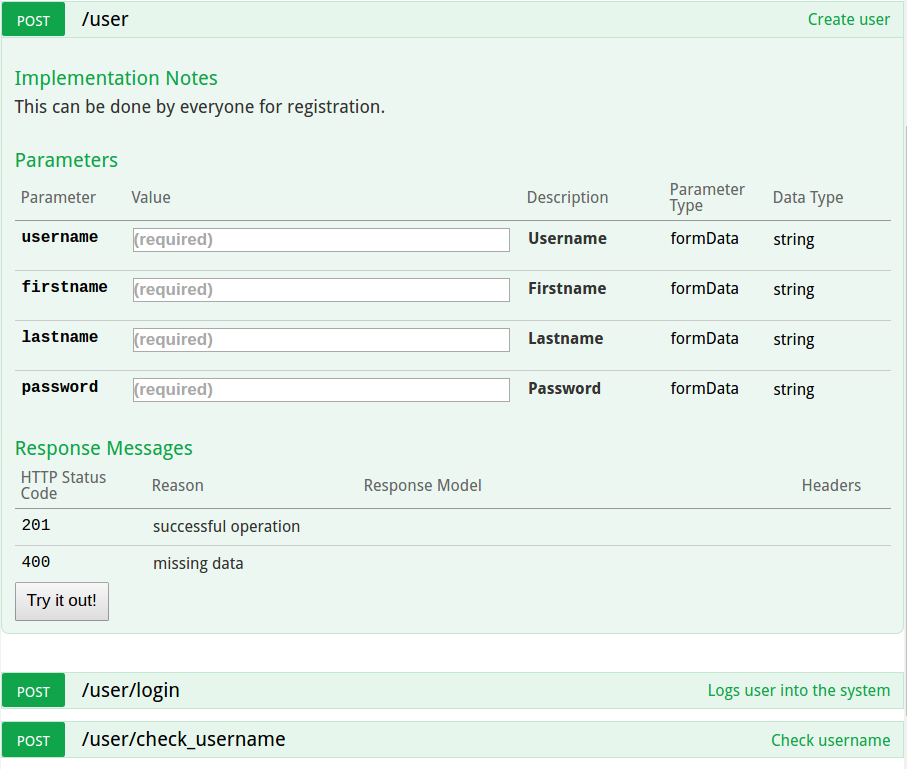
\includegraphics[width=1\textwidth]{API/user_02.png} 
\caption{Documentazione per login e registrazione}
\label{fig:user:login}
\end{figure}

\section{FUN-03}
Il terzo requisito funzionale prevede di dare la possibilità agli utenti dell'app di segnalare nuovi beacon.
Per fare ciò l'app ha bisogno di sapere dal server quali beacon sono già stati segnalati.
Troviamo quindi una rotta che ci permette di recuperare l'elenco di tutti i beacon che sono già stati segnalati.

\begin{lstlisting}[caption={/webserver/app/routes/beacon.js get}, style=javaScriptCode]
  //Everybody can access to beacon list
  router.get('/', function(req, res) {
    Beacon.find({},function(err, beacons) {
      if(err) {
        res.status(500).send({msg: err.errmsg});
      } else if(beacons && beacons.length>0) {
        res.status(200).send(beacons);
      } else {
        res.status(200).send([]);
      }
    });
  });
\end{lstlisting}
Inoltre l'app ha bisogno anche di una seconda rotta per salvare il beacon nel backend.
Questa volta, però, l'operazione potrà essere effettuata soltanto da chi ha già effettuato il login.
\begin{lstlisting}[caption={/webserver/app/routes/beacon.js aggiunta}, style=javaScriptCode]
  //User must be logged to add new beacon
  router.post('/', function(req, res) {
    if(req.user.block) {
      res.status(401).send({'msg': 'Authentication required'});
    } else if(!req.body.uuid || !req.body.major || !req.body.minor){
      res.status(400).send({'msg': 'Missing data'});
    } else {
      var newBeacon = new Beacon({
        uuid: req.body.uuid,
        major: req.body.major,
        minor: req.body.minor
      });
      newBeacon.save(function (err) {
        if(err) {
          res.status(500).send({msg: err.errmsg});
        } else {
          res.status(201).send({'msg': 'ok'});
        }
      });
    }
  });
\end{lstlisting}

Come potete osservare dalla documentazione la richiesta dei beacon deve essere fatta in GET mentre l'aggiunta in POST.

\begin{figure}[h]
\centering
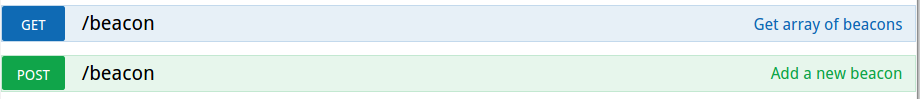
\includegraphics[width=1\textwidth]{API/beacon_03.png} 
\caption{Documentazione richieste beacon}
\label{fig:beacon}
\end{figure}

\section{FUN-04}
Il quarto requisito prevede la possibilità di ricercare i server di Proximity System all'interno della propria LAN.
Per fare ciò abbiamo dato la possibilità al client di pingare ogni singolo host all'interno della propria rete con una specifica rotta.
In modo tale che il client, a seconda se il server risponde correttamente o meno, sappia se quell'indirizzo è di un server PS.
La rotta in questione è la seguente.
\begin{figure}[h]
\centering
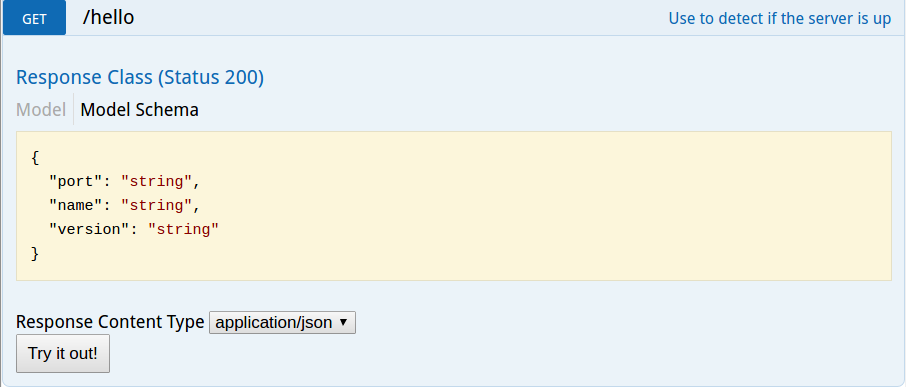
\includegraphics[width=1\textwidth]{API/setting_hello.png} 
\caption{Documentazione per hello}
\label{fig:user:login}
\end{figure}
Come si può dedurre dalla documentazione, il codice è molti semplice.
\begin{lstlisting}[caption={/webserver/app/routes/setting.js hello}, style=javaScriptCode]
  router.get('/hello', function(req, res) {
    var response = {
      port: "8000",
      name: "ProximitySystem",
      version: "2.0"
    };
    res.status(200).send(response);
  });
\end{lstlisting}
Per il momento le informazioni sono statiche per tutti i server, ma in futuro è possibile che queste informazioni saranno personalizzabili.

\section{FUN-05/07}
I requisiti funzionali dal 05 al 07 non interessano il backend.
Per questo motivo si rimanda alla tesi di Marco per maggiori informazioni.
\section{FUN-08}
L'ottavo requisito funzionale prevede il controllo manuale dei GPIO da parte dell'admin.
Un GPIO(General Purpose Input Output) è un piedino del RaspberryPI che o è configurato per pilotare un relè oppure per ricevere un input da un sensore.
La gestione manuale di essi permette sia di pilotare i relè manualmente, dando la possibilità all'amministratore di spegnere/accendere i dispositivi associati in qualsiasi momento, sia di leggere i relativi input collegati.
Per questo motivo abbiamo previsto due rotte.

\begin{figure}[h]
\centering
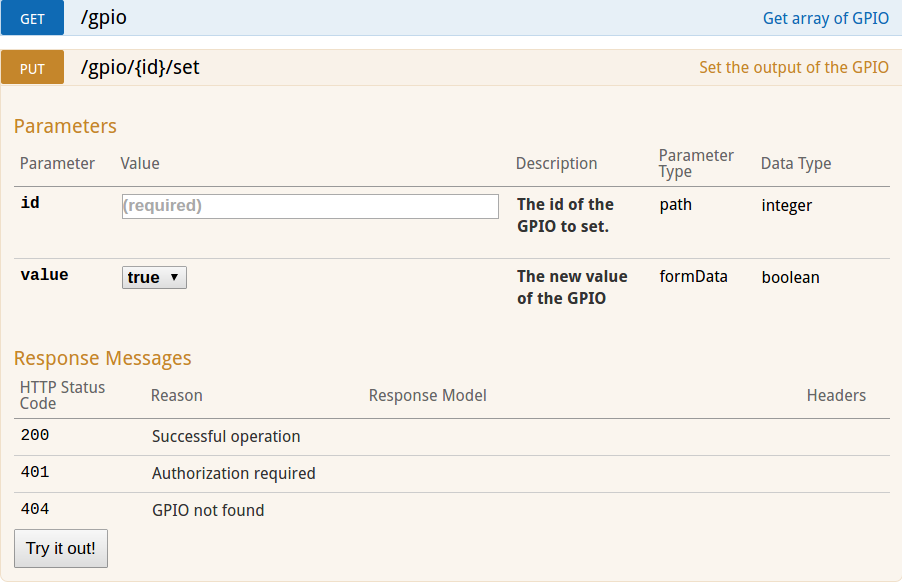
\includegraphics[width=1\textwidth]{API/gpio.png} 
\caption{Documentazione per la gestione dei GPIO}
\label{fig:user:login}
\end{figure}

Una di lettura, che permette di avere le informazioni di tutti i GPIO, sia di input che di output
(ovviamente questa operazione è permessa solo agli admin).

\begin{lstlisting}[caption={/webserver/app/routes/gpio.js get}, style=javaScriptCode]
  router.get('/', function(req, res) {
    if(req.user.block || req.user.permission !== 0) {
      res.status(403).send({'msg':'Forbidden'});
    } else {
      GPIO.find(function(err, GPIOs) {
        if(err) {
          res.status(500).send({msg: err.errmsg});
        } else if(GPIOs) {
          res.status(200).send(GPIOs);
        }
      });
    }
  });
\end{lstlisting}

Una di scrittura, che permette di settare i GPIO di output a false o a true.

\begin{lstlisting}[caption={/webserver/app/routes/gpio.js set}, style=javaScriptCode]
  router.put('/:id/set', function(req, res) {
    if(req.user.block || req.user.permission !== 0) {
      res.status(403).send({'msg':'Forbidden'});
    } else {
      GPIO.findOne({
        '_id': req.params.id,
        'type':'output'
      }, function(err, gpio) {
        if(err) {
          res.status(500).send({'msg': err.msg});
        } else if(gpio) {
          if(undefined != req.body.value) {
            gpio.value = req.body.value;
          }
          gpio.save(function (err) {
            if(err) {
              res.status(500).send({msg: err.errmsg});
            } else {
              pin.setPin(gpio.GPIO, gpio.value, function(err) {
                if (err) {
                  res.status(500).send('Oops, Something went wrong! ' + err);
                } else {
                  io.emit('update:gpio');
                  io.emit('update:device');
                  res.status(200).send(gpio);
                }
              }, environment);
            }
          });
        } else {
          res.status(404).send({'msg': 'Not found'});
        }
      });
    }
  });
\end{lstlisting}

Anche in questo caso possiamo notare l'utilizzo delle websocket per notificare a tutti i client che delle informazioni importanti sono state aggiornate.
Oltre a questo, e alle classiche callback a cascata, possiamo notare che la chiamata setPin accetta un paramatro che si chiama environment.
Questo parametro indica al sistema se ci troviamo in fase di sviluppo oppure in produzione, ovvero nel Raspberry.
Nel primo caso la chiamata al GPIO sarà semplicemente simulata.

\section{FUN-09/10/11}
I requisiti funzionali 09, 10 e 11 verranno trattati insieme anche se rappresentano la gestione di componenti diverse del sistema(utenti e dispositivi) perché a livello di API la funzioni di cui abbiamo bisogno sono molto simili tra loro. 
Infatti, le singole operazioni effettueranno la modifica di una singola collection del database.
In realtà, sono molto simili anche alle rotte viste precedentemente, motivo per cui mostreremo solamente la documentazione delle rotte implementate.

\begin{figure}[h]
\centering
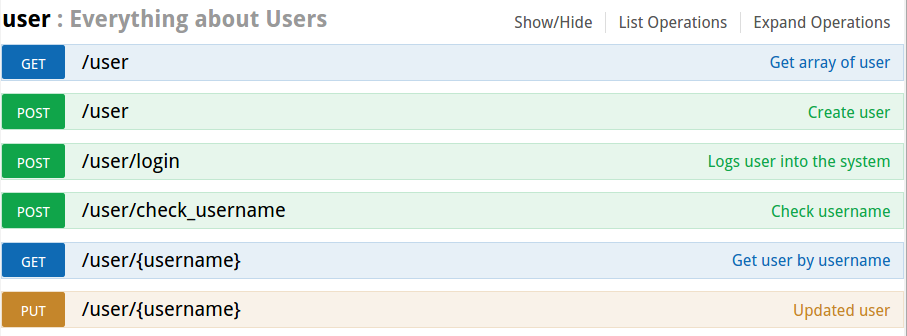
\includegraphics[width=1\textwidth]{API/user.png} 
\caption{Documentazione per la gestione degli utenti}
\label{fig:user}
\end{figure}

Nella figura \ref{fig:user} sono presenti tutte le rotte per la gestione degli utenti comprese quelle per il login e la registrazione.
I restanti tre metodi(due in GET ed uno in POST) sono accessibili solo all'admin e permettono di modificare i dati dei vari utenti.

\begin{figure}[h]
\centering
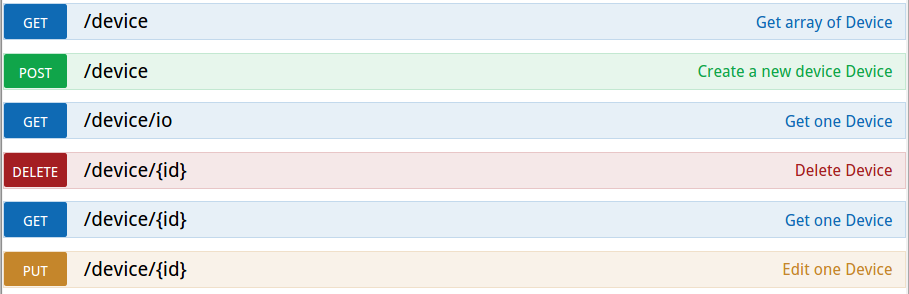
\includegraphics[width=1\textwidth]{API/device.png} 
\caption{Documentazione per la gestione dei dispositivi}
\label{fig:device}
\end{figure}

Per la gestione dei dispositivi le API sono molto simili a quelle degli utenti.
L'unica aggiunta è una rotta per l'eliminazione di un dispositivo.

\section{FUN-12/13/14}
Gli ultimi tre requisiti funzionali descrivono come i vari componenti devono comunicare tra loro.
Il RaspberryPi deve poter interagire con il mondo esterno grazie all'utilizzo di relè e sensori.
Sia l'app che la WebApp devono comunicare con il backend tramite il protocollo HTTP.
L'app deve essere l'unico componente che è in grado di ricevere i messaggi bluetooth inviati dai beacon.
Tutto questo viene sintetizzato nel seguente Deployment Diagram.
\begin{figure}[h]
\centering
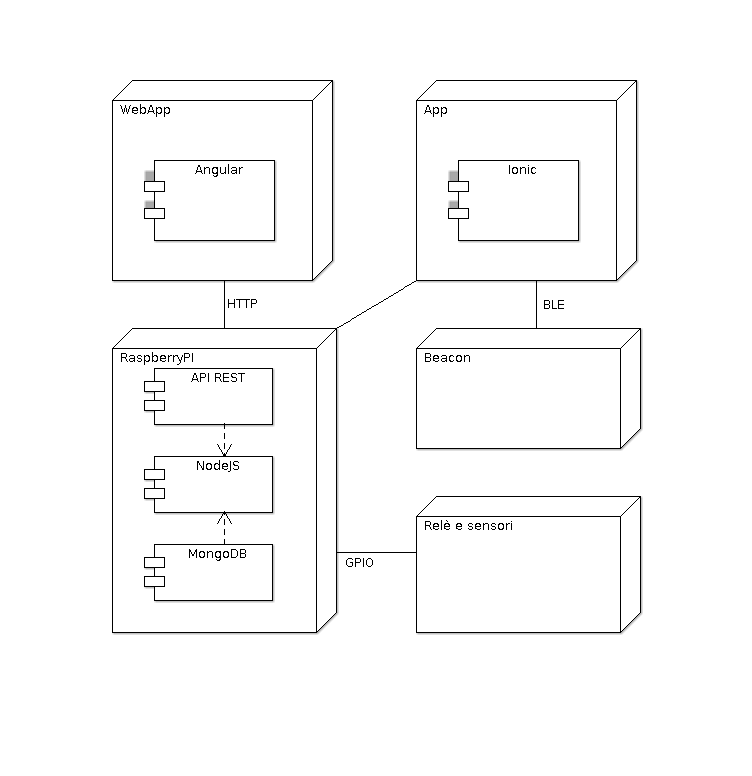
\includegraphics[width=1\textwidth]{DeploymentDiagram.png} 
\caption{Deployment Diagram}
\label{fig:deployment}
\end{figure}
\chapter{Conclusioni}
\label{chap:conc}

Lo scopo di questa tesi era la realizzazione di un prototipo per la domotica d'ufficio che prevedesse l'utilizzo dei beacon.
Al di la della parte pratica di tutto ciò, siamo andati a trattare diverse tecnologie che si stanno sviluppando in questi ultimi anni, sia a livello software che a livello hardware.

Abbiamo visto come il linguaggio JavaScript sia passato da essere utilizzato per l'esecuzione di qualche controllo nelle pagine web tipico degli anni 90, a essere un linguaggio di riferimento per lo sviluppo di applicazioni sia sul front-end che sul back-end.
Infatti, grazie a Node, JavaScript è stato portato anche sui server, diventando un linguaggio universale. 
Per universale intendo la capacità di un programma di essere eseguito su qualsiasi dispositivo indipendentemente dal sistema operativo utilizzato e dall'hardware sottostante.

Abbiamo introdotto l'utilizzo di database documentali al posto di quelli relazionali evidenziandole le principali differenze.
In particolare, grazie all'assenza di una struttura vera e propria, i database documentali sono più adatti in progetti in cui il software viene sviluppato in maniera incrementale.

Con l'introduzione delle WebSocket abbiamo visto una delle tante specifiche introdotte con l'HTML5 che sta rivoluzionando il web.
Grazie a questa, ed altre importanti novità, un programmatore ha tutti gli strumenti necessari per sviluppare un'applicazione da far girare all'interno del proprio browser che ha veramente poco, se non nulla, da invidiare ad una applicazione desktop tradizionale.
   
Per quanto riguarda l'hardware, i beacon sono dispositivi semplici ma allo stesso tempo si possono rivelare molto utili in alcuni contesti come il marketing. 
Al contrario di come molti pensano, i beacon non comunicano informazioni dirette alle app. 
Sono le applicazioni che rilevano la vicinanza di un determinato beacon e una volta identificato eseguono un'azione.
Nel nostro caso specifico, quando uno smartphone con l'app installata rileva di essere entrato nella regione di un beacon invia un comando per pilotare il dispositivo associato.
Nel caso vengano utilizzati per una campagna di marketing, quando uno smartphone rileva un beacon sa di essere nella vicinanze di un determinato negozio, può scaricare dal server le relative promozioni e inviare una notifica all'utente con le offerte più adatte a lui.

    
\section{Il futuro di Proximity System}

Una volta completato il nostro prototipo, con l'aiuto di extrategy e in particolare Silvia Morresi, abbiamo realizzato il modello di business del nostro prodotto.
Per modello di business si intende l'insieme delle soluzioni organizzative e strategiche attraverso le quali l'impresa acquisisce vantaggio competitivo.
Per fare ciò, abbiamo utilizzato uno strumento che utilizza il linguaggio visuale per realizzare modelli di business innovativi: \textbf{Il Business Model Canvas}.
Grazie a questo framework e alla sua efficacia comunicativa tutti possono comprendere elementi complessi che riguardano il funzionamento di un'azienda.

Le descrizioni dettagliate del nostro modello di business e del BMC in generale verranno fatte nella tesi di Marco. 
Per ora, eccovi un'anteprima:
\begin{figure}[htpb!]
  \centering
  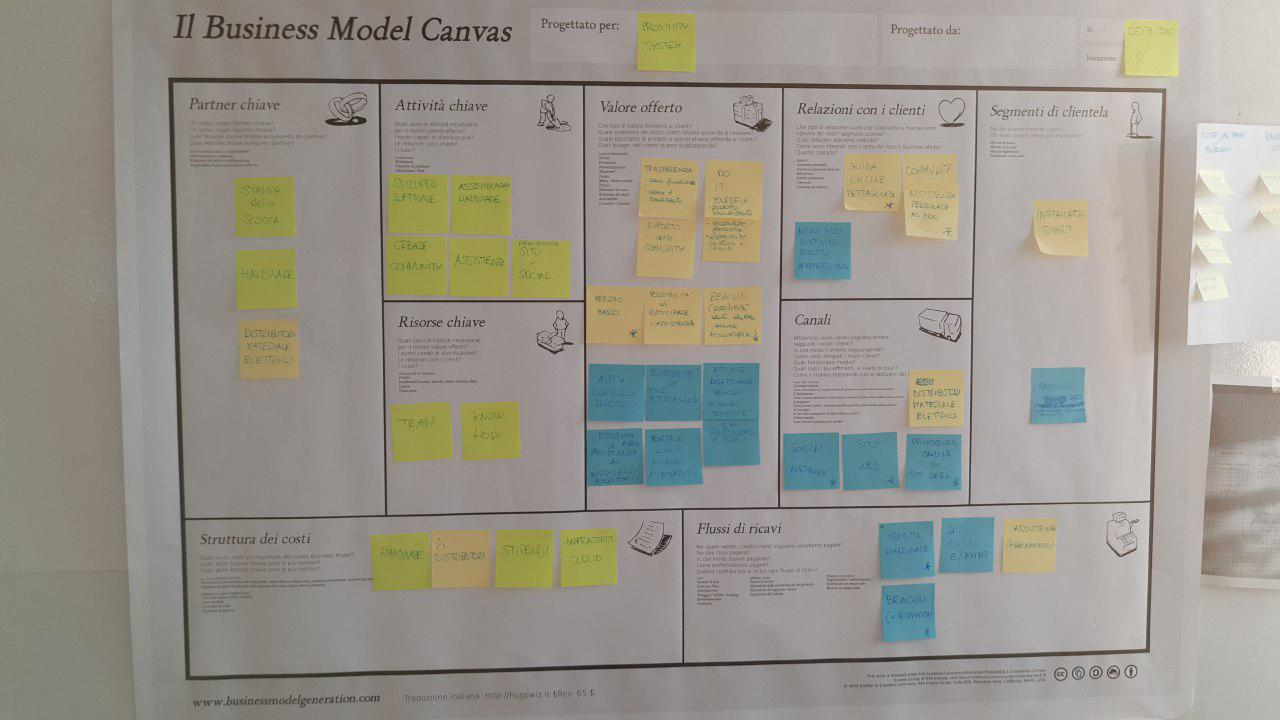
\includegraphics[width=1\textwidth]{bmc}
  \caption{Il nostro Business Model Canvas}
  \label{fig:bmc}
\end{figure}


\appendix
%\chapter{Schema elettrico}
\section{Modifica dell'impianto}
\begin{figure}
\centering
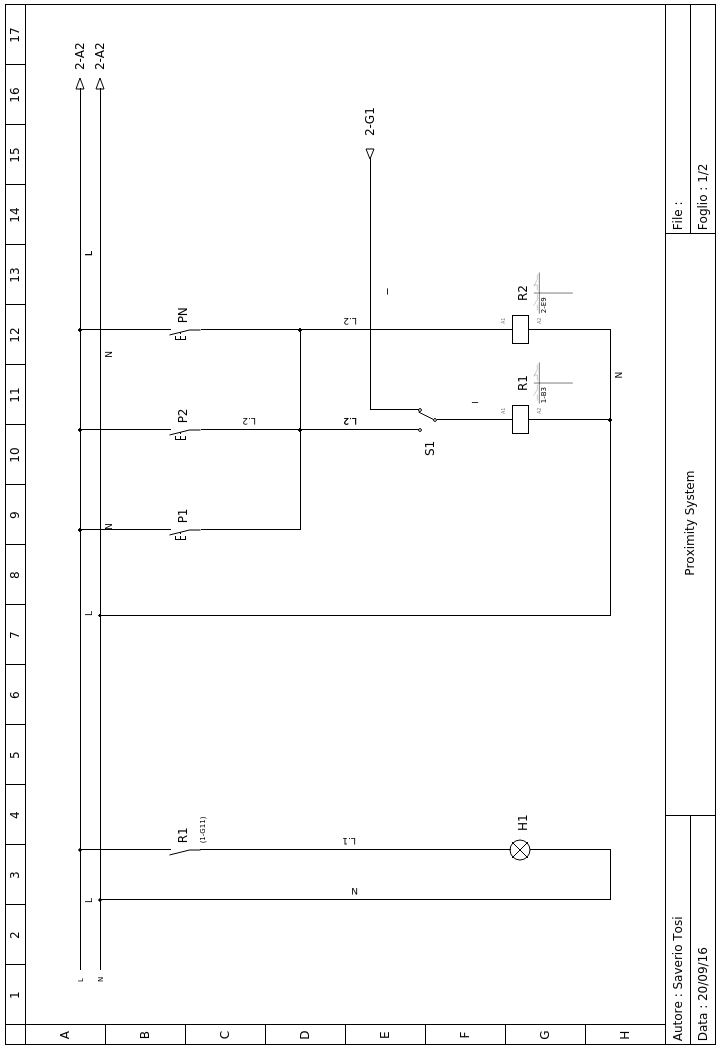
\includegraphics[scale=0.57]{Immagini/schema_p1.png}
\end{figure}
\begin{figure}
\centering
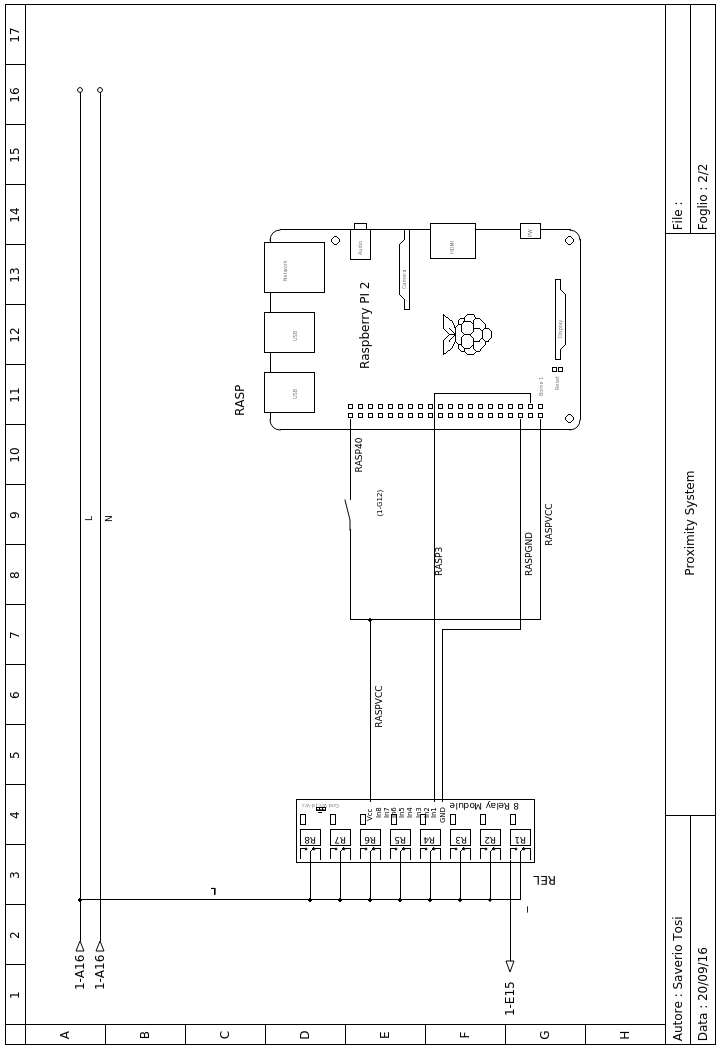
\includegraphics[scale=0.57]{Immagini/schema_p2.png}
\end{figure}
\chapter{Installazione Proximity System}
\chapter{Screenshot Proximity System}
\section{App}
\begin{figure}[htpb!]
  \centering
  \subfloat[][\emph{Home page dell'app}.]
  {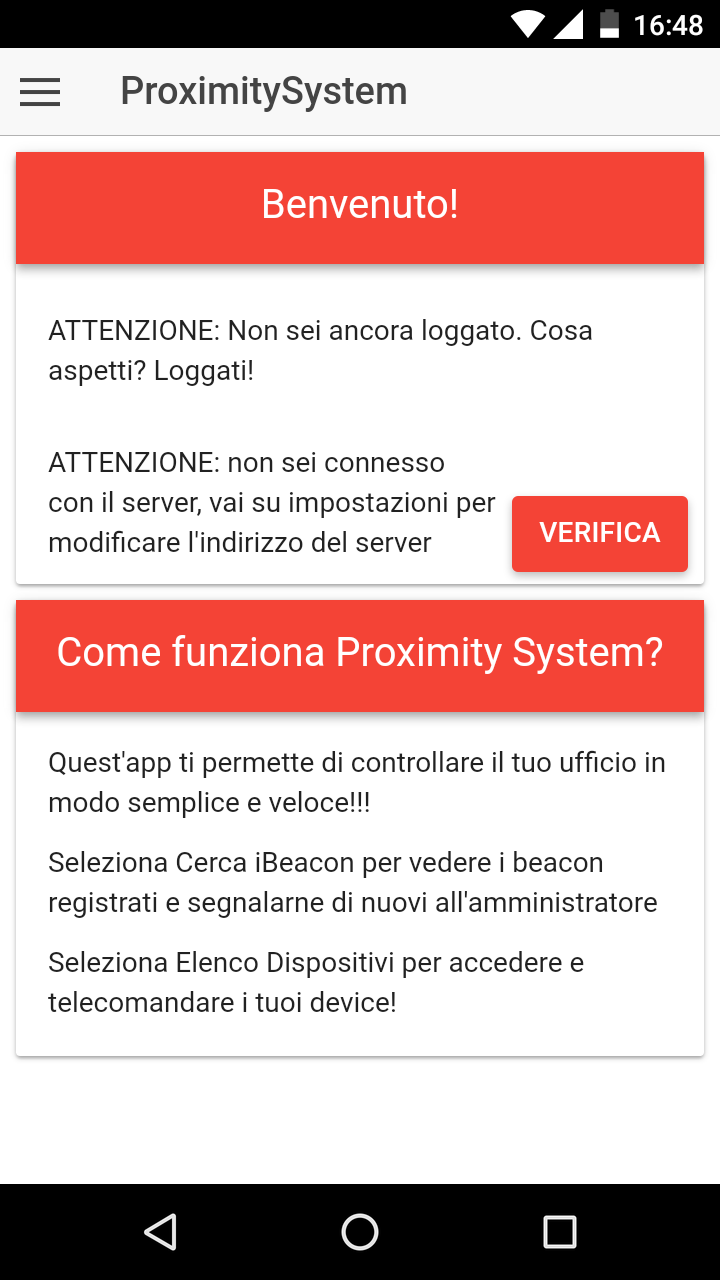
\includegraphics[width=.4\textwidth]{ionic_start}} \quad
  \subfloat[][\emph{Ricerca di server}.]
  {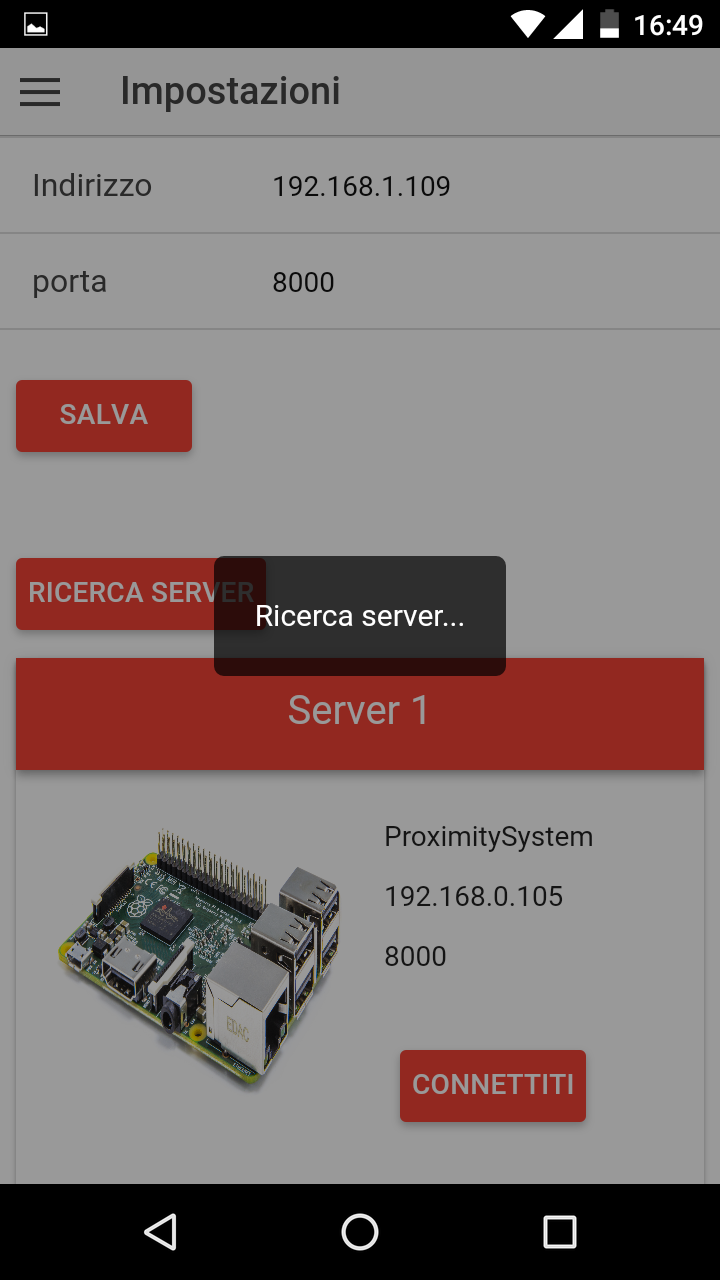
\includegraphics[width=.4\textwidth]{ionic_ricerca}} 
  \caption{Connessione iniziale con il server di Proximity System.}
  \label{fig:subfig}
\end{figure}

\begin{figure}
  \centering
  \subfloat[][\emph{Registrazione nuovo account}.]
  {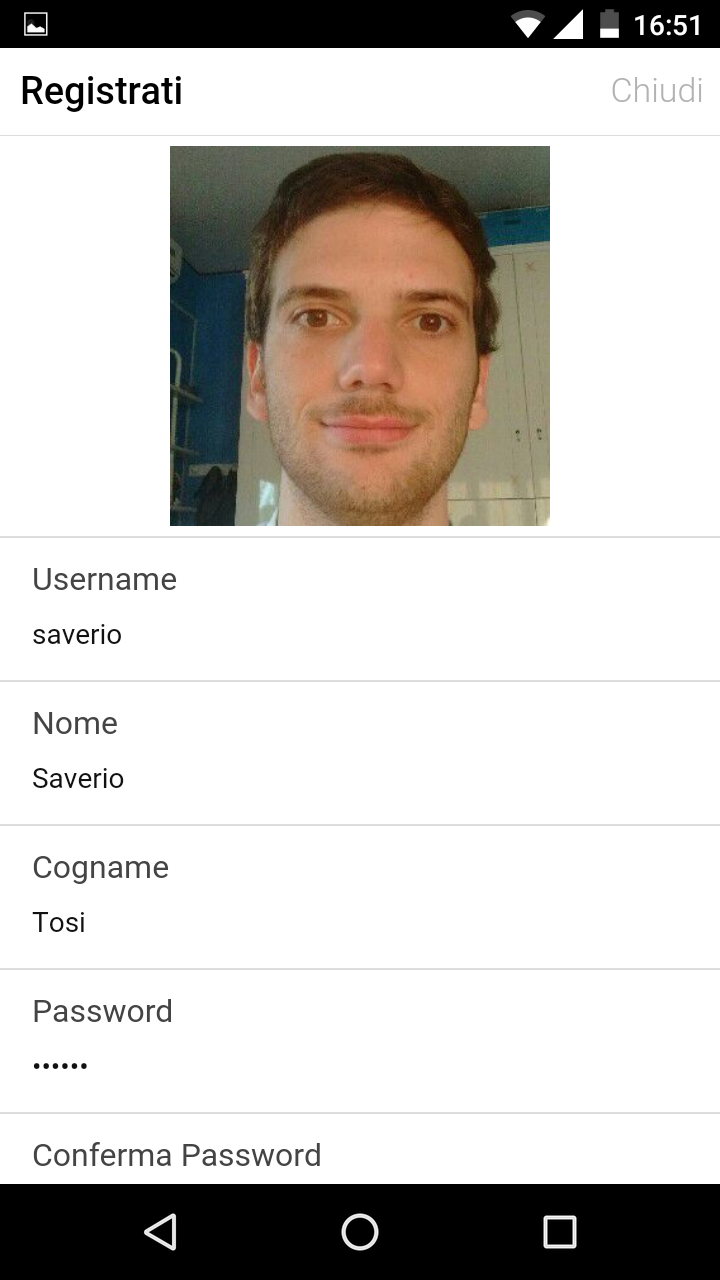
\includegraphics[width=.4\textwidth]{ionic_registrazione}} \quad
  \subfloat[][\emph{Login dall'app}.]
  {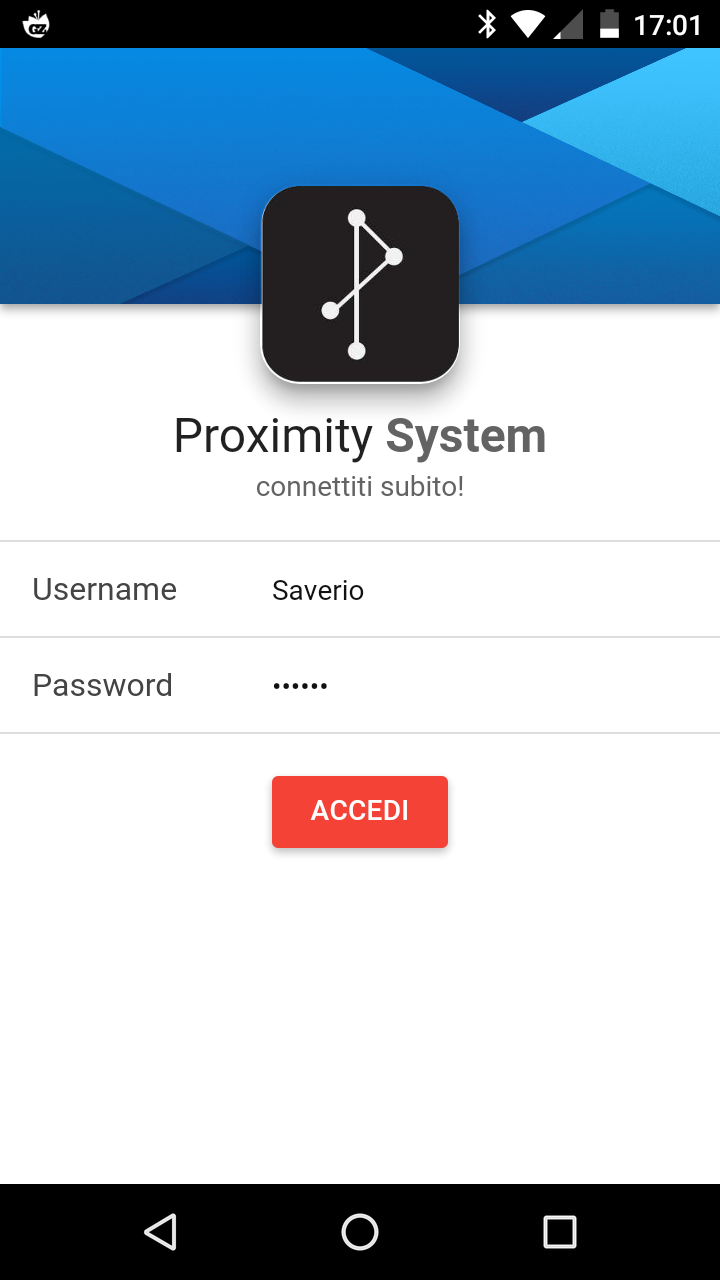
\includegraphics[width=.4\textwidth]{ionic_login}} \\
  \subfloat[][\emph{Ricerca nuovi beacon}.]
  {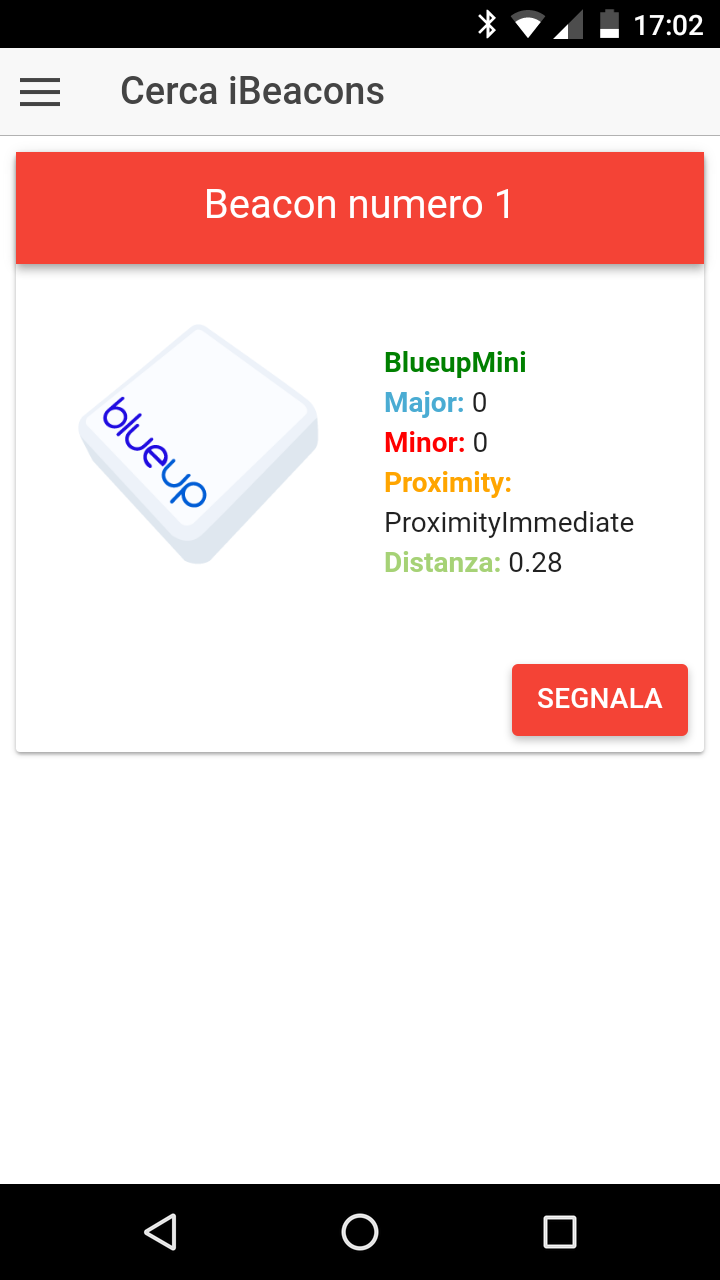
\includegraphics[width=.4\textwidth]{ionic_beacon}} \quad
  \subfloat[][\emph{Elenco dei dispositivi}.]
  {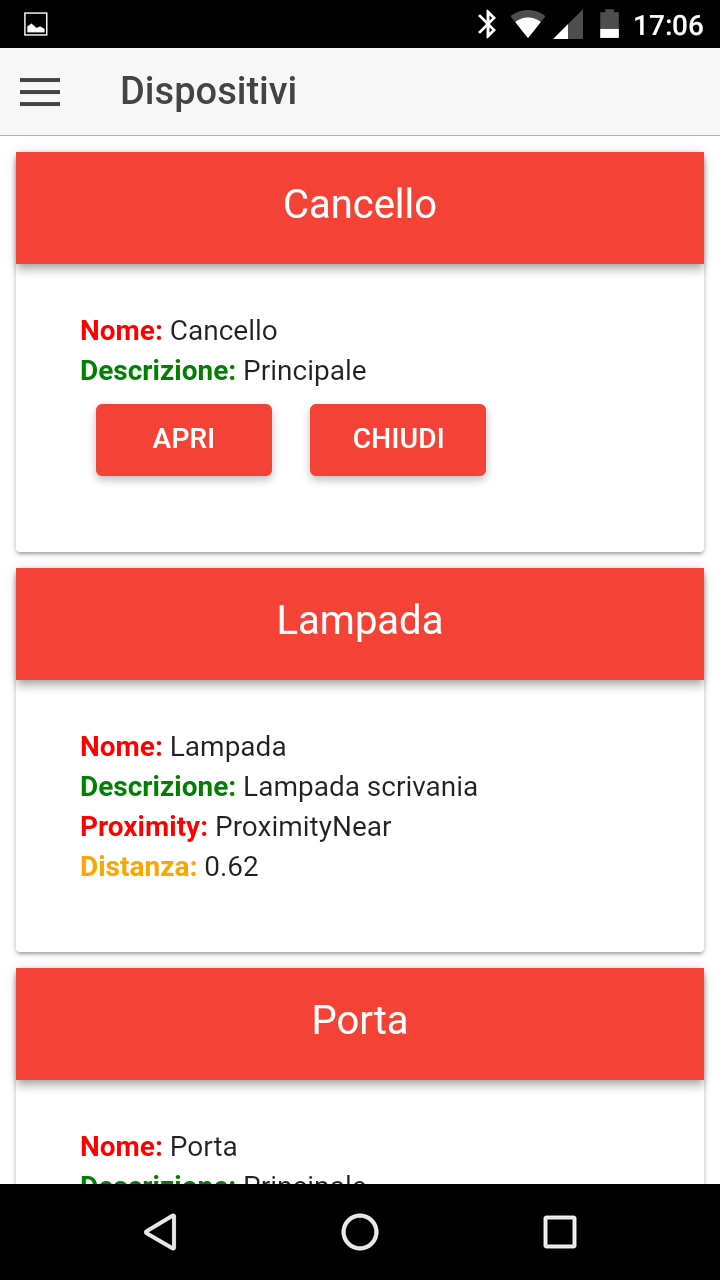
\includegraphics[width=.4\textwidth]{ionic_dispositivi}} 
  \caption{Alcune delle pagine principali dell'app.}
  \label{fig:subfig}
\end{figure}

\section{WebApp}

\begin{figure}[htpb!]
  \centering
  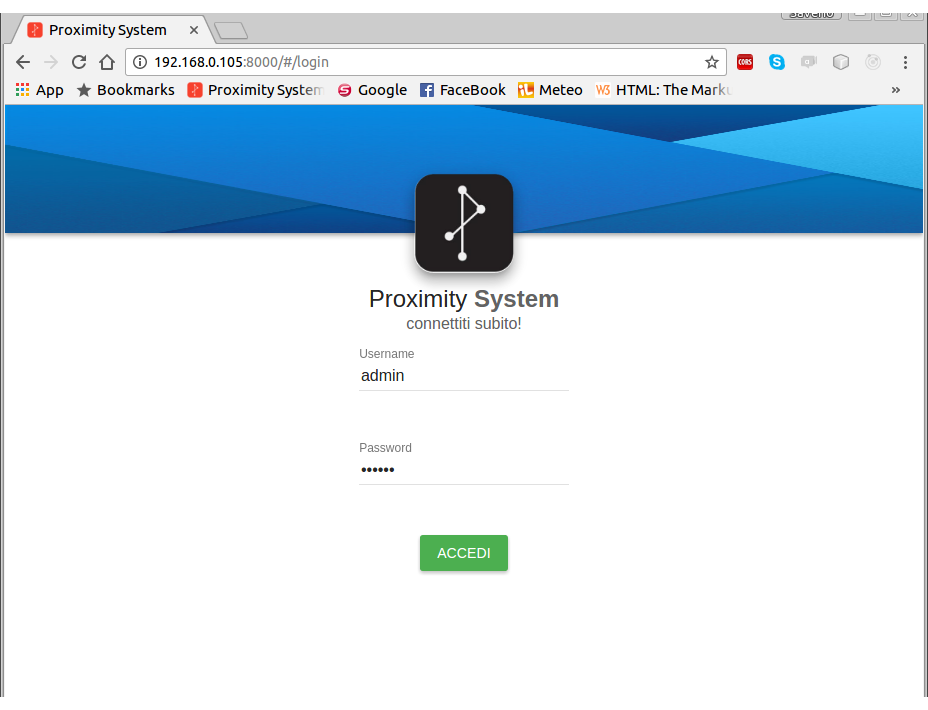
\includegraphics[width=0.8\textwidth]{login}
  \caption{Login da webapp}
  \label{fig:login}
\end{figure}

\begin{figure}[htpb!]
  \centering
  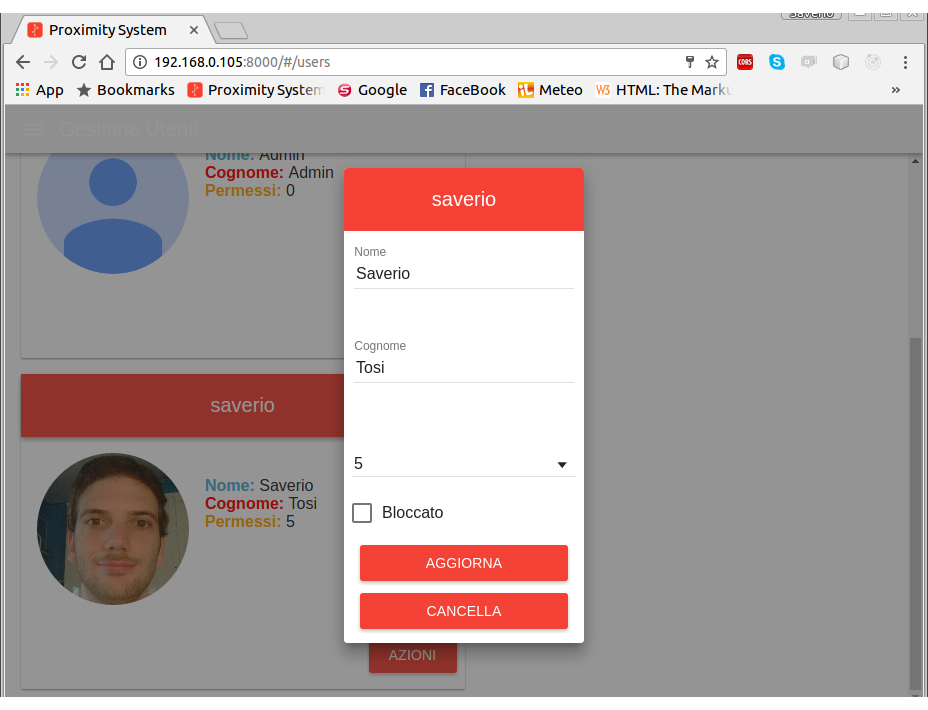
\includegraphics[width=0.8\textwidth]{utenti}
  \caption{Gestione utenti}
  \label{fig:utenti}
\end{figure}

\begin{figure}[htpb!]
  \centering
  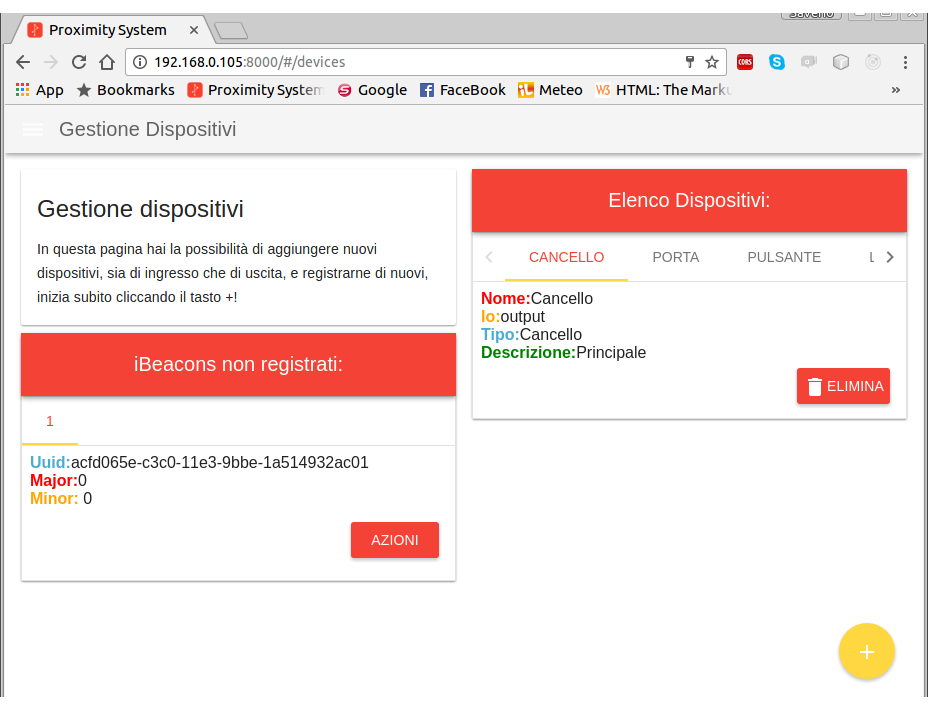
\includegraphics[width=0.8\textwidth]{dispositivi}
  \caption{Gestione dispositivi}
  \label{fig:dispositivi}
\end{figure}

\begin{figure}[htpb!]
  \centering
  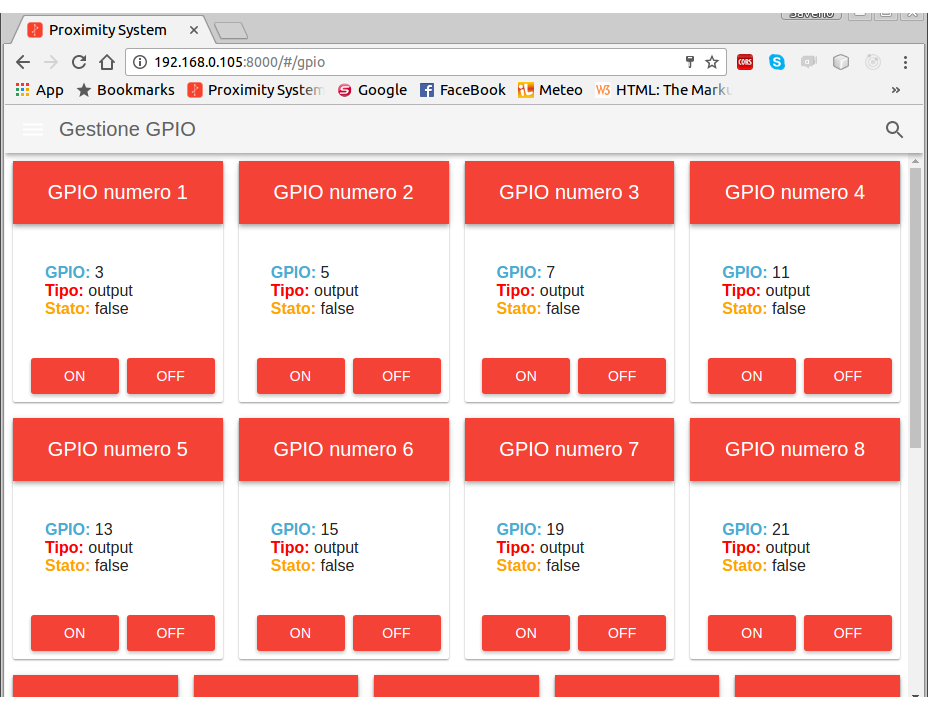
\includegraphics[width=0.8\textwidth]{gpio}
  \caption{Gestione GPIO}
  \label{fig:gpio}
\end{figure}

\begin{figure}[htpb!]
  \centering
  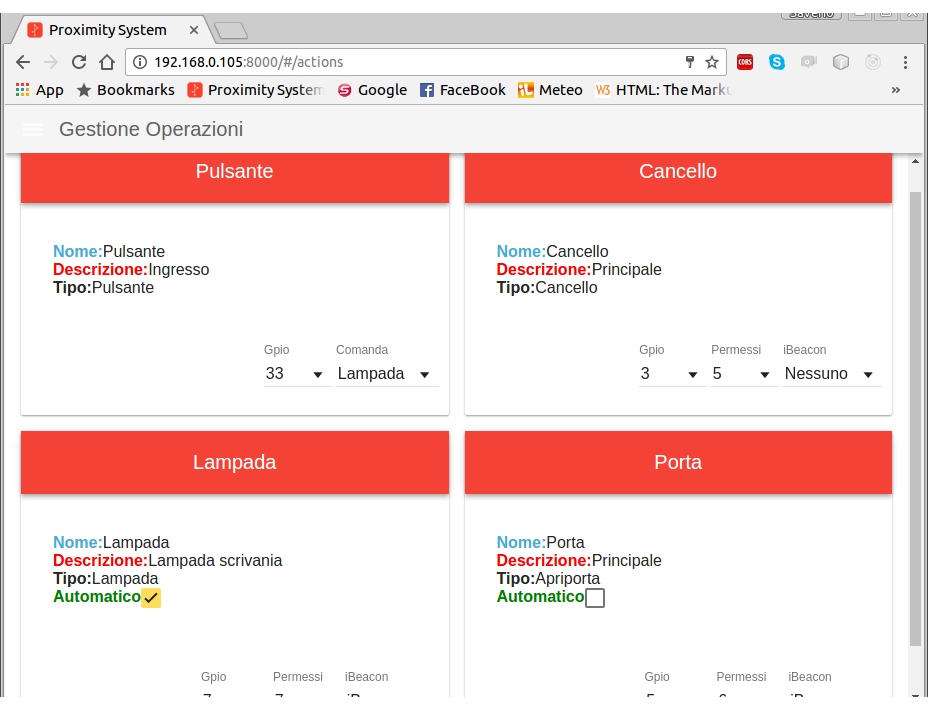
\includegraphics[width=0.8\textwidth]{operazioni}
  \caption{Gestione operazioni}
  \label{fig:operazioni}
\end{figure}

\printbibliography

\printindex
\chapter*{Ringraziamenti}

\end{document}